\documentclass[12pt,a4paper]{report}
%\documentclass[a4paper]{report}
\usepackage{alltt}
\usepackage{listings}
\usepackage{caption}
\usepackage{url}
\usepackage{amsthm}
\usepackage{setspace}
\usepackage{graphicx}
\newtheorem{definition}{Definition}[chapter]
\usepackage[top=2.5cm, bottom=2.5cm, left=2.5cm, right=2.5cm]{geometry}
%\usepackage{courier}
%\renewcommand{\ttdefault}{pcr}
%\usepackage[T1]{fontenc}
%\usepackage{courier}
%\renewcommand*\familydefault{\ttdefault}

\DeclareGraphicsExtensions{.pdf}
\graphicspath{{./diagrams/}}

\begin{document}

\lstset{
  basicstyle=\small\ttfamily,           % the size of the fonts that are used for the code
%  frame=lines,
  numberstyle=\footnotesize,      % the size of the fonts that are used for the line-numbers
  stepnumber=2,                   % the step between two line-numbers. If it is 1, each line 
  % will be numbered
  numbersep=5pt,                  % how far the line-numbers are from the code
  showspaces=false,               % show spaces adding particular underscores
  showstringspaces=false,         % underline spaces within strings
  showtabs=false,                 % show tabs within strings adding particular underscores
  tabsize=4,                      % sets default tabsize to 2 spaces
  captionpos=b,                   % sets the caption-position to bottom
  breaklines=true,                % sets automatic line breaking
  xleftmargin=20pt,
  xrightmargin=20pt,
  breakatwhitespace=false,        % sets if automatic breaks should only happen at whitespace
  title=\lstname,                 % show the filename of files included with \lstinputlisting;
  escapeinside={\%*}{*)},         % if you want to add a comment within your code
  morekeywords={*,...}            % if you want to add more keywords to the set
}

\lstdefinelanguage{LLVM}
  {morekeywords={define, ret, call, load, add, sub, store, switch, bitcast,
  ptrtoint, inttoptr, label, global, undef},
  sensitive=false,
  morecomment=[l]{;},
  morestring=[b]",
}

\lstdefinelanguage{Haskell}
  {morekeywords={data, type, where, let, Just, Nothing, deriving, Show, letrec,
  in},
  sensitive=true,
  morecomment=[l]{;},
  morestring=[b]",
}


\lstdefinestyle{assembler}{
  language=LLVM
}
\lstdefinestyle{haskell}{
  language=Haskell
}

\title{Kivi: Lazy functional programming language targeting Low Level Virtual Machine}
\author{\textit{Author:}\\Piotr Micha\l{} Kaleta\\\\\emph{Supervisor:}\\dr W\l{}odzimierz Moczurad}
\date{\today}

\maketitle

\newpage
\thispagestyle{empty}
\mbox{}

\onehalfspace

\Huge
\begin{abstract}
  \normalsize
  \center
  This paper describes the design and implementation of a new lazy programming
  language called Kivi. It is based on the concept of \textit{G-machine}, an
  efficient implementation of graph reducer. Kivi's syntax resembles the one of
  Haskell, but beneath syntactic layer, it differs significantly. The code that
  Kivi generates, is the intermediate language of a compiler toolkit called
  \textit{Low Level Virtual Machine}\cite{website:llvm} or \textit{LLVM} for
  short.  Later LLVM compiles and assembles the program into an executable.
  Programs written in Kivi are therefore likely to gain run-time speed-ups due
  to highly developed optimization mechanisms implemented in LLVM. Choosing
  LLVM as a backend makes it easier to port programs to different architectures
  as well.  Kivi is meant to form the basis of a future implementation of a
  lazy language for concurrent programming, integrated with Erlang by means of
  its distribution protocols.
\end{abstract}

\normalsize

\pagenumbering{roman}
\tableofcontents

\pagenumbering{arabic}
\chapter{Introduction}

This paper describes the design and implementation of a lazy functional
language compiler. The implementation is based on the
\textit{G-machine}\cite{Jon87} and uses \textit{lazy graph reduction} to
perform evaluation. Current compiler, attached to this thesis, is implemented
in Haskell, however in future I'm planning to reimplement it using Kivi itself,
thus exploiting a technique called \textit{bootstrapping} (see
\cite{wiki:bootstrapping}).

The compilation process is implemented as a set of passes that eventually
transforms source code written in Kivi into a simple intermediate language
, \textit{lambda calculus} enriched with let(rec) expressions. Choice to
implement it by several passes was mainly motivated by readability concerns, as
well as the will to make implementation and debugging as easy as possible.
Another reason for this might be the fact that such separation made the
compiler very modular and adding another pass should be done with minimal
complexity.

Following chapter presents the parsing mechanisms used in Kivi. It is a description
of lexical and syntax analysers that translate code written in Kivi into an
abstract construct, which is used throughout the whole futher compilation
process.

Another chapter provides a description of translation processes that eventually
transform source code into \textit{enriched lambda calculus}, a variant of
lambda calculus with several differences like added let(rec) expressions and
supercombinators. Later, enriched lambda calculus is going to be converted
into \textit{G-code}, a sequence of instructions that can be executed on
G-machine.

Third chapter shows an implementation type-checker, which is used to ensure
that certain kind of type errors cannot occur during run-time of a Kivi
program. It also performs a \textit{type inference}, that deduces the types
that has previously been omitted in Kivi's source.

The last part of this thesis forms a description of G-machine. It presents the
general execution model, as well as gives two implementations. The first one is
an interpreter, whereas the second one is a LLVM intermediate representation
code generator.

\chapter{Parsing}

In order to translate the source of \textit{Kivi} into \textit{Lambda Calculus}
it has to be available in a structured form so thate next passes could easily
traverse it. \textit{Abstract Syntax Trees}\cite{ALSU07} has been widely
adopted as a standard form of keeping the representation of source code in
memory. The process of reading the input source file and producing AST from it
is called \textit{parsing}.

I have chosen to implement a simple parser, in a similar manner as in
\cite{JonLes00} as it seemed to be the simplest approach to me back then. Now, as
the parser has grown, I would strongly consider rewriting it to use parser
combinator library such as \cite{website:parsec} instead.

Parsing consists of two passes:

\begin{itemize}
  \item Firstly \textit{lexical analysis} implemented by \texttt{lex} in
    \textit{Lexer.hs} module extracts \textit{tokens} from plain text.
    \textit{Tokenization} is the process of demarcating and possibly
    classifying sections of a string of input characters. The resulting tokens
    are then passed on to further processing.
  \item \textit{Syntax analysis} is the process of analyzing the stream of
    tokens and building an \textit{Abstract Syntax Tree} from it.
\end{itemize}

This process is implemented as\footnote{Where \texttt{PatProgram} is a program
that contains patterns}:

\vspace*{0.2in}
\begin{lstlisting}
parse :: String -> PatProgram
parse = syntax . lex
\end{lstlisting}

And can be seen as presented in Figure~\ref{fig:parser}.

\vspace*{0.2in}
\begin{figure}[h!]
  \centering
  \includegraphics[height=9cm]{parser}
  \caption{Parser schema.}
  \label{fig:parser}
\end{figure}

\section{Lexical analysis}

The types for lexer are following:

\vspace*{0.2in}
\begin{lstlisting}
type Token = String
type TokenInfo = (Int, Token)
\end{lstlisting}
Where \texttt{TokenInfo} consist of line number and a token string itself.

The heart of lexical analyser is the \texttt{lex'} function. It works by
classifying the parts of remaining input based on first characters.  Building
number tokens may be a nice example of how it works:

\vspace*{0.2in}
\begin{lstlisting}[label=lst:lex_comment,caption={Building tokens from numbers.}]
lex' (c : cs) lnum | isDigit c =
    (lnum, numToken) : lex' restCs lnum
    where
        numToken = c : takeWhile isDigit cs
        restCs = dropWhile isDigit cs
\end{lstlisting}


\section{Syntax analysis}
\label{sec:syntax_analysis}
Once lexer is capable of emitting tokens, it is time to convert it into a
hierarchical structure called \textit{Abstract Syntax Tree} (or \textit{AST}
for short). Abstract syntax trees are tree representations of abstract
syntactic structures written in programming language. Nodes in such tree
represent different constructs from the source code. The word abstract is used
because not every detail from source code has its corresponding piece in AST,
some unnecessary details are ommited.

Data type for representing Kivi's abstract syntax trees is defined in
\textit{Common.hs} module and is a parametrized data type. This concept is
similar to templates in C++ or generics in Java. It allows the code to be
reused and is an important ingredient in \textit{parametric poylmorphism}, the
way that Haskell achieves polymorphism (see
\cite{website:parametric_polymorphism}). The data type definition is following:

\vspace*{0.2in}
\begin{lstlisting}
data Expr a = EVar Name
            | ENum Int
            | EChar Int
            | EConstrName Name
            | EConstr Int Int
            | EAp (Expr a) (Expr a)
            | ELet IsRec [Defn a] (Expr a)
            | ECase (Expr a) [Alter Pattern a]
            | ECaseSimple (Expr a) [Alter Int a]
            | ECaseConstr (Expr a) [Alter Int a]
            | ELam [a] (Expr a)
            | EError String
            | ESelect Int Int Name
\end{lstlisting}
The \texttt{Expr} data type is parametrized with respect to its binders.
Binders, as name suggests, are used when the variable is bound to a value. This
happens in lambda abstractions, let and letrec definitions as well as in
case expressions. To give an example of how a simple source code
construct will look like, when parsed to AST, consider the following
snippet of code:

\vspace*{0.2in}
\begin{lstlisting}
let
    x = 1;
    y = 2
in
    x + y
\end{lstlisting}
The result returned from \texttt{parse} function will be\footnote{In reality
the output from \texttt{parse} is more complicated because it returns programs
with patterns. However in order to grasp the concept of parametrized
\texttt{Expr} type its easier to forget about that fact for a while.}:

\vspace*{0.2in}
\begin{lstlisting}
  ELet False
       [('x', ENum 1), ('y', ENum 2)]
       EAp (EAp (EVar '+') (EVar 'x')) (EVar 'y')
\end{lstlisting}

Defining expressions in this way makes the code way more concise. For example,
initially parser returns programs with patterns in them, but later phases of
compilation process gets rid of them by transforming program into a
representation that uses \texttt{case} expressions instead. Thanks to
parametrized definition of \texttt{Expr} data type, it is possible to define
parse as function that returns \texttt{Expr Pattern}, whereas subsequent phases
return \texttt{Expr String}.


\chapter{Translation to Lambda Calculus}

In this chapter I am going to present the process of transforming a high-level
functional language into a simple intermediate form called \textit{lambda calculus}.
In the first part I will show \textit{Kivi}'s syntax, its constructs and
structures. Later on, the desired output form, \textit{Lambda Calculus} will be
shown. The rest of the chapter will focus on methods to translate the first form
into another.

\section{Syntax}
Sources of Kivi programs consist of set of
\textit{supercombinators}\cite{wiki:supercombinator}. Supercombinator is an
expression consisting of either constants or other supercombinators and does
not contain any free variables (see Definition~\ref{def:free_variable}) in its
body. Supercombinators might have arguments but those which does not, are
called \textit{constant applicative forms} (or \textit{CAF}s for short).
Listing~\ref{supercombinator_ex} shows the simple supercombinator with one
argument, calculating square of a given number.

\vspace*{0.2in}
\begin{lstlisting}[style=haskell,label=supercombinator_ex,caption={Simple supercombinator.}]
sqr x = x * x
\end{lstlisting}

There exists one distinguished supercombinator called \textit{main}, that takes
no arguments. It is the entry point for program execution. If there is no main
CAF present in Kivi's source, both compiler and interpreter should issue a
specific error message.

\subsection{Case expressions}
The purpose of case expressions is to allow the programmer to control the flow
of program execution via a multiway branch. The semantics of case is rather
simple. First, the expression under case is evaluated and then, based on result,
the appriopriate execution path is chosen. Example of case expression is
presented in Listing~\ref{lst:case_expression}.

\vspace*{0.2in}
\begin{lstlisting}[style=haskell,label=lst:case_expression,caption={Fibonacci with case}]
fib n =
    case n of
        0 -> 1;
        1 -> 1;
        n -> fib (n-1) + fib (n-2);

main = fib 10
\end{lstlisting}

\subsection{If expressions}
Reason for if expressions to exist, is to make the life easier for programmers
coming from imperative languages, for if expressions can be implemented using
case ones, without changing its semantics, and this is the recommended
approach.  In fact what Kivi does under the hood is to translate if to case.
What is different from most imperative languages, is the fact that ifs are
expressions, not statements, therefore they return a value. If expressions
takes an expression that should evaluate to boolean value, as well as two
expressions that are returned if the value under test is true or
false:

\vspace*{0.2in}
\begin{lstlisting}[style=haskell,label=lst:if_expression,caption={Fibonacci with case}]
f x = if (x > 100) x (x * x)
\end{lstlisting}

\subsection{Local bindings}
Supercombinators provides the ability to define local definitions using
\texttt{let} keyword. The scope of variables defined using \texttt{let} is
enclosed by the expression following \texttt{in} keyword. The example use of
local binding is presented in Listing~\ref{let_ex}

\vspace*{0.2in}
\begin{lstlisting}[style=haskell,label=let_ex,caption={Local \texttt{let} binding.}]
sum x y = x + y;

main =
    let x = 1
        y = 2
    in
        sum x y
\end{lstlisting}

\subsection{Recursive local bindings}
In order to define recursive bindings, one has to use a special \texttt{letrec}
construct as shown in Listing~\ref{factorial_letrec_ex}

\vspace*{0.2in}
\begin{lstlisting}[style=haskell,label=factorial_letrec_ex,caption={Factorial function using \texttt{letrec}.}]
sum x y = x + y;

main =
    letrec fac n =
        case n == 0 of
            True  -> 1;
            False -> n * fac (n-1)
    in
        fac 5
\end{lstlisting}

\subsection{Where clauses}
Another way of creating recursive definitions is using the \texttt{where}
clause. Internally it will be translated into letrec binding. Example use of
\texttt{where} clause is shown in Listing~\ref{factorial_where_ex}

\vspace*{0.2in}
\begin{lstlisting}[style=haskell,label=factorial_where_ex,caption={Factorial function using \texttt{where}.}]
main = fac 5
    where
        fac n = case n == 0 of
            True  -> 1;
            False -> n * fac (n - 1)
\end{lstlisting}

\subsection{Lambda abstractions}
Functions in Kivi can be defined in two ways. The first one is the top level
supercombinators that has already been discussed. The other option is to define
them as \textit{lambda abstractions}. This concept is similar to \textit{anonymous
functions} used in imperative languages. The syntax for defining lambda
abstractions is presented in Listing~\ref{lambda_ex}.

\vspace*{0.2in}
\begin{lstlisting}[style=haskell,label=lambda_ex,caption={Lambda abstraction}]
f = (\x . x * 2) 42
\end{lstlisting}

In this example the lambda abstraction which doubles the arguments value is
created and then applied to 42 yielding 84 as result.

During compilation process programs containing lambda abstractions are
transformed into their equivalents with lambda abstractions substituted for top
level supercombinators. This process is called \textit{lambda lifting} and is
described in more detail in chapter~\ref{sec:lambda_lifting}.

\subsection{Pattern matching}

Pattern matching consists of specifying patterns to which some data should
conform and then checking to see if it does, as well as deconstructing the data
according to those patterns. So in other words, using pattern matching you can
recognize values, bind variables to those values and break structures down into
parts.
Patterns are matched in order they are defined in source code. Once a
successful branch is found, the right-hand-side expression is evaluated and
result returned. None of the following patterns is checked. If after checking
all patterns it turns out that none of them matches the argument, the error is
returned.

\vspace*{0.2in}
\begin{lstlisting}[style=haskell,label=pattern_matching_ex,caption={Factorial using pattern matching.}]
fac 0 = 1
fac n = n * fac (n - 1)
\end{lstlisting}

In Listing~\ref{pattern_matching_ex} a recursive supercombinator \texttt{fac}
calculating factorial is defined. There are two cases\footnote{To be honest
there are three cases, but for simplicity reasons we assume that
\texttt{fac} is called only for non-negative integers}. Either the
argument is 0 and then the result is 1, or argument is other than than 0 and
then we progress recursively. The factorial definition is expressed very
clearly by means of pattern matching.
Pattern matching is also very useful when it comes to dealing with data
types as we will see in next section.

\subsection{Structured Data Types}
Data types in Kivi are defined using \texttt{data} keyword, giving the name of
new type as well as its constructors and arities. Together with pattern matching they
provide a very powerful mechanism for dealing with structured entities.

\vspace*{0.2in}
\begin{lstlisting}[style=haskell,label=data_type_ex,caption={Calculating length of list.}]
data List = Nil 0 | Cons 2;

length Nil = 0;
length (Cons x xs) = 1 + length xs
\end{lstlisting}

In Listing~\ref{data_type_ex} a data type \texttt{List} is declared as well as
supercombinator calculating the length of a list by means of pattern matching.
In first case argument is pattern matched to the \texttt{Nil} constructor. If
matching succeeds it means that the list is empty, therefore its length is 0.
In next case the argument is matched to second \texttt{List} constructor, that
is \texttt{Cons}. If argument matches, the \textit{tail} of the list is bound to
\texttt{xs} variable and right hand side of that branch is evaluated.

\subsection{Partial function application}
It is possible to create \textit{partial function applications} also known as
\textit{currying}. It means that supplying an argument to a function, yields
another function of smaller arity. Given a function $f : A \times B \rightarrow
D$ and fixing the first argument creates a function $f : B \rightarrow C$. An
example is presented below:

\vspace*{0.2in}
\begin{lstlisting}[style=haskell,caption={Partial application of addition.}]
add a b = a + b;
add3 = add 3;
main = add3 4
\end{lstlisting}

\section{Translation to Lambda Calculus}
The process of translating a high-level functional language to \textit{lambda
calculus} might be considered as a set of program transformations. Each such
transformation is meant to simplify \footnote{or help with further
transformations} the program given as its input, eventually leading to the
expected \textit{enriched lambda calculus} form. All these transformations
accept one form of program as input and yield the transformed program as
output. We might, therefore, regard the compilation process as a function
composition of all transformations. This is exactly the way the compilation is
implemented in Kivi, and Haskell provides means to express this in a very
concise way:

\vspace*{0.2in}
\begin{lstlisting}[style=haskell]
run :: String -> String
run = showResults
    . eval
    . compile
    . analyseDeps
    . lambdaLift
    . lazyLambdaLift
    . transformToLambdaCalculus
    . mergePatterns
    . tag
    . parse
\end{lstlisting}

We have already discussed parsing in previous chapters, so in the following
sections I am going to provide a description of all remaining phases.

\section{Structured Data Types and Tagging}
In order to understand the need for this pass one has to know how structured
data types and their constructors are represented internally.
A custom data type declaration in Kivi might look like this one:

\vspace*{0.2in}
\begin{lstlisting}[style=haskell]
data Tree = Leaf 1 | Branch 2
\end{lstlisting}

This statement declares the new data type called \texttt{Tree} which can be
constructed in two ways. The common way of looking at the constructors is to
consider them as functions with zero or more arguments that return an instance
of a data type as a result. The \texttt{Tree} constructor is \texttt{Leaf} and
it has no further descendants. It takes one argument which is some kind of
value. The other way to construct a \texttt{Tree} is to create a \texttt{Branch}
taking two children (which also are \texttt{Tree}s) as arguments. For example,
conceptual representation of the following tree is shown in Figure~\ref{fig:tree}:

\vspace*{0.2in}
\begin{lstlisting}[style=haskell]
Branch (Leaf 1) (Branch (Leaf 2) (Leaf 3))
\end{lstlisting}

\begin{figure}[h!]
  \centering
  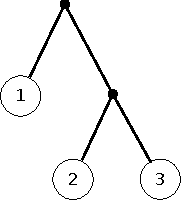
\includegraphics[height=4cm]{tree}
  \caption{Tree built using abstract data types.}
  \label{fig:tree}
\end{figure}

Constructors are used not only for object creation but also for decomposition
into parts as well as distinguishing the different types of trees based on
constructor. This feature is heavily used when pattern matching. For example
the code in Listing~\ref{lst:sqr_tree} uses it to create a new tree with values
that are square roots of values in original tree.

\vspace*{0.2in}
\begin{lstlisting}[label=lst:sqr_tree,caption={Creating a `square rooted` tree.}]
sqrTree (Leaf v) = Leaf (v * v)
sqrTree (Branch t1 t2) = Branch (sqrTree t1) (sqrTree t2)
\end{lstlisting}

\subsection{Built-in Data Types}
There are few types that are considered built-ins. These are lists, tuples,
and booleans. The ability to think of these common concepts in functional
programming as Structured Data Types makes the implementation straightforward
as I did not have to treat these entities separately, instead I used a common
notion of data types.
\subsubsection{Booleans}
Boolean values in Kivi are implemented as a regular Structured Data Type having
two constructors representing true and false:

\vspace*{0.2in}
\begin{lstlisting}[style=haskell]
data Boolean = True | False
\end{lstlisting}

\subsubsection{Lists}
Lists are structures that allow storing a number of items. They
provide a set of operations on them that allowing to create other
lists\footnote{In Kivi lists as well as other types are immutable, which means
that you cannot modify its contents. Instead you create new values which may
differ from previous ones. }
Kivi provides a variety of way to define a list. First of all lists can be seen
as regular Data Type. Thus there are two constructors for a \texttt{List}
data type. \texttt{Nil} and \texttt{Cons}:

\vspace*{0.2in}
\begin{lstlisting}[style=haskell]
data List = Nil 0 | Cons 2
\end{lstlisting}

\texttt{Nil} instantiates an empty \texttt{List} whereas \texttt{Cons} is meant
to \textit{construct} \texttt{List} given two elements: the \textit{head} and
\textit{tail}. List are recursive structures, thus \textit{tail} is another
list.

It turns out that creating a \texttt{List} is a task that occurs very often in
functional languages, therefore it would be nice not to have to write long
constructs such as this one to create 4-element \texttt{List}:

\vspace*{0.2in}
\begin{lstlisting}[style=haskell]
Cons 1 (Cons 2 (Cons 3 (Cons 4 Nil)))
\end{lstlisting}

Most functional languages allow programmer to express it in a much shorter way,
and Kivi does it too:

\vspace*{0.2in}
\begin{lstlisting}[style=haskell]
[1, 2, 3, 4]
\end{lstlisting}

The same thing concern constructing lists given two elements. Kivi provides
`:`(colon) as construction operator for \texttt{List} type, so the programmer
would write:

\vspace*{0.2in}
\begin{lstlisting}[style=haskell]
((2+3) : [1,2,3,4])
\end{lstlisting}
instead of:

\vspace*{0.2in}
\begin{lstlisting}[style=haskell]
Cons (2+3)  [1,2,3,4]
\end{lstlisting}

\subsubsection{Tuples}
Tuples are yet another way of storing multiple values in a single one. However
the difference between them and lists is significant. Tuples are
\textit{immutable} in a way that you cannot \textit{cons} to a tuple nor
decompose them into parts using pattern matching. Their main usage is when a
programmer knows in advance how many elements will he need to store.

There is a predefined number of tuple types that you can create, and currently
the bound is set to 4. This means that programmer is not allowed to create
tuples that contain more than 4 elements. This design decision is due to the
fact that from my perspective it is better to use custom structured data type
for readability reasons. The limit of 4 however, is an experimental value and
might be changed.

This all means that tuples with different number of elements are different
types. Therefore there is no such thing as generic `Tuple` type. There are
however \texttt{Tuple0}, \texttt{Tuple1}, \ldots etc., representing tuples with
0 elements, 1 element, \ldots etc.

There are two ways to create a tuple either by using constructors or by a
special \textit{syntactic sugar} construct, similarly as in the case for lists.
These two ways for instantiating a 3-element tuple are equivalent, with the
preference for the second one, due to readability concerns:

\vspace*{0.2in}
\begin{lstlisting}[style=haskell]
(((Tuple3 1) 2) 3)
\end{lstlisting}
and

\vspace*{0.2in}
\begin{lstlisting}[style=haskell]
(1, 2, 3)
\end{lstlisting}

\subsection{Implementation and tagging}
Internally each data type consist of a list of constructors, each containing a
\textit{tag}, and \textit{arity}. Constructor tags should uniquely identify
each constructor therefore each tag should be different. The definitions
for \texttt{DataType} and \texttt{Constructor} type synonyms, as in
\textit{Common.hs} are as follows:

\vspace*{0.2in}
\begin{lstlisting}[style=haskell]
type DataType = (Name, [Constructor])
type Constructor = (Name, Int, Int)
\end{lstlisting}

Because of the fact that there is no way to know in advance how many data type
declarations are there in source file I had to devise some way to assign a
unique tag for each of constructors that is not a built-in one. This is
precisely what the tagging phase is for. It works in two parts:

\begin{itemize}
  \item First it traverses the list of data types and its constructors in order
    to create a mapping between constructor name and its unique tag.
  \item Next the whole AST is recursively traversed and each
    \texttt{EConstrName} node is substituted for \texttt{EConstr} containing
    the previously associated tag and arity.
\end{itemize}

The definitions for those functionalities has been placed in
\textit{AbstractDataTypes.hs} file. This module also contains functionalities
responsible for querying constructors for tags, names, arities as well as
finding constructors given the \texttt{DataType} instance.


\section{Pattern Matching}
This section describes the details and motivation behing pattern matching as
well as describes details of algorithms that transform high-level pattern
matching constructs into enriched lambda calculus.

\vspace*{0.2in}
\begin{lstlisting}[style=haskell,label=lst:length,caption={Calculating length of list.}]
length [] = 0;
length (x : xs) = length xs + 1

length Nil = 0;
length (Cons x xs) = length xs + 1
\end{lstlisting}

Listing~\ref{lst:length} reminds the already well known function for
calculating the length of a list, and also presents the version of the same
function but without \textit{syntactic sugar}. For the purpose of further
discussion lets assume that we are calculating the length of 3-element list:

\vspace*{0.2in}
\begin{lstlisting}[style=haskell]
[1, 2, 3]
\end{lstlisting}
which is the same as:

\vspace*{0.2in}
\begin{lstlisting}[style=haskell]
Cons 1 (Cons 2 (Cons 3 Nil))
\end{lstlisting}

The way the pattern matching compiler works, is that when length is applied to
an expression it might be not evaluated yet, so in order to proceed we have to
evaluate the function argument. Next, compiler checks whether argument is a Nil
constructor. This is not the case so compiler proceeds to checking against the
second branch. This time it succeeds and \texttt{x} is bound to \texttt{1} and
\texttt{xs} is bound to \texttt{[2, 3]}. The left-hand-sides of function
equations are called \textit{patterns}. They can consist of constructors,
variables, numbers, single characters and strings\footnote{Both the built-in
ones as well as those defined by programmer.}. In previous example we have seen
the combination of those, i.e. The pattern was composed of constructors and
variables. Nothing prevents programmer from creating the so called
\textit{nested patterns}. Example of such situation is present in
Listing~\ref{lst:second_element}, where the function is extracting the second
element from the list.

\vspace*{0.2in}
\begin{lstlisting}[style=haskell,label=lst:second_element,caption={Greatest common divisor.}]
second [] = 0;
second [x] = 0;
second (x1 : (x2 : xs)) = x2
\end{lstlisting}

Patterns in the previous example were not \textit{overlapping}. It
means that changing the order of function equations would not alter the
behaviour of the function. The situation changes when we look at example
presented in Listing~\ref{lst:gcd}.

\vspace*{0.2in}
\begin{lstlisting}[style=haskell,label=lst:gcd,caption={Greatest common divisor.}]
gcd a 0 = a;
gcd a b = gcd b (b % a)
\end{lstlisting}

Here if we have changed the order of equations, the function will never terminate
because the first clause would always match. This kind of patterns are called
\textit{overlapping patterns}.

Pattern matching can occur not only in function equations but also in source
code constructs. It can be used in \texttt{case} expressions as well as in
let and letrec bindings. Examples of those two pattern
matching uses are presented in Listing~\ref{lst:case_pattern_matching} and
~\ref{lst:letrec_pattern_matching}.  Making pattern matching available in
let(rec)s at first sight might look like very similar to other constructs. In
reality, however, it requires quite a complicated additional pass that
transform let(rec)s into more suitable form.  This transformation is described
in more detail in Section~\ref{sec:letrec_transform}.

\vspace*{0.2in}
\begin{lstlisting}[style=haskell,label=lst:case_pattern_matching,caption={Pattern matching in
case expressions.}]
sqrList list =
    case list of
        [] -> []
        (x : xs) -> ((x * x) : sqrList xs)
\end{lstlisting}

\vspace*{0.2in}
\begin{lstlisting}[style=haskell,label=lst:letrec_pattern_matching,caption={Pattern matching
  in let(rec) expressions.}]
let
    (x : xs) = [1, 2, 3, 4];
    (y : ys) = [5, 6, 7, 8]
in
    x + y
\end{lstlisting}

\subsection{Compiling Pattern Matching}
The simplest way to think of pattern matching is to match expression with first
pattern and in case it does not match, try the following patterns. Within each
equation patterns are tested from left to right\footnote{In case of functions
with multiple patterns}. Lets consider an example of \texttt{map} function from
Listing~\ref{lst:map}.

\vspace*{0.2in}
\begin{lstlisting}[style=haskell,label=lst:map,caption={Map function example.}]
map f [] = [];
map f (x : xs) = ((f x) : (map f xs));

main = map (\x . x * x) [1, 2, 3, 4, 5]
\end{lstlisting}

The \texttt{map} function returns a list constructed by appling a function
\texttt{f} to all items in a list passed as the second argument. What our
mental model of pattern matching will do when evaluating the \texttt{main}
function, is that it will first try to match the \texttt{(\textbackslash x . x
* x)} lambda abstraction with \texttt{f} variable which will succeed. Matching
any expression to variable will result in success. Then the list \texttt{[1, 2,
3, 4, 5]} will be matched against an empty list - \texttt{[]} and it will fail.
In this situation, according to our simple strategy the algorithm will try to
match the second equation. So it will again try to match the lambda abstraction
with \texttt{f} variable pattern. As we can observe evaluation according to the
simple algorithm might result in redundant computations, and in case of more
complicated patterns it might be a substantial drawback. In order to be able to
perform pattern matching in more optimized fashion we have to transform into
the following form:

\vspace*{0.2in}
\begin{lstlisting}[style=haskell,mathescape=true]
map = $\lambda$f.$\lambda$xs.
    case xs of
        Nil       -> Nil
        Cons y ys -> Cons (f y) (map f ys)
\end{lstlisting}

The remaining part of this section contains a description of an algorithm that
is capable of transforming pattern matching into the form that uses case
expressions instead of \textit{pattern-matching lambda abstractions}, thus allowing to
compile patterns more efficiently. In order to see a more detailed analysis
refer to Chapters 4 and 5 of \cite{Jon87}.

\subsection{Pattern-matching Lambda Abstractions}
In lambda calculus, regular lambda abstraction is an expression of the
following form:

\vspace*{0.2in}
\begin{lstlisting}[style=haskell,mathescape=true]
$\lambda x.t$
\end{lstlisting}
where \textit{x} represents a \textit{variable} and \textit{t} stands for
\textit{term}. Intuitively, a lambda abstraction is an anonymous function that
takes a single input, and the \(\lambda\) is said to bind \textit{x} in
\textit{t}, and an application \textit{ts} represents the application of input
\textit{s} to some function \textit{t}. In the lambda calculus, functions are
taken to be first class values, so functions may be used as the inputs to other
functions, and functions may return functions as their outputs.

The difference between regular and pattern-matching lambda abstractions lies in
a fact that instead of variable $x$ on the left side a pattern might be
used. So it might look like that:

\vspace*{0.2in}
\begin{lstlisting}[style=haskell,mathescape=true]
$\lambda p.t$
\end{lstlisting}
where $p$ is a pattern\footnote{Variable is also considered as a
pattern, so regular lambda abstractions form a subset of pattern-matching ones.}

\subsection{Free variables}
\label{sec:free_variable}

For the purpose of further deliberations I will present the definition of
\textit{free variables}:
\begin{definition}
  \label{def:free_variable}
  A free variable is a notation that specifies places in an expression where
  substitution may take place. The idea is related to a placeholder (a symbol
  that will later be replaced by some literal string), or a wildcard character
  that stands for an unspecified symbol.
\end{definition}

In computer programming, a free variable is a variable referred to in a
function that is not a local variable nor an argument of that function:

\subsection{Translating function equations to pattern-matching lambda
abstractions}
For the purpose of further explanations lets consider the following function
definition:

\vspace*{0.2in}
\begin{lstlisting}[style=haskell,mathescape=true]
$f\:p_{1} = e_{1}$
$f\:p_{2} = e_{2}$
   $\vdots$
$f\:p_{n} = e_{n}$
\end{lstlisting}

The pattern matching will be executed from top to bottom until some of them
matches or none of them matches. In the first situation the value of an
expression on the right hand side of matched pattern should be returned and
none of the following patterns should be matched against. In the second one an
error should be reported that no matching branch was found. With this in mind
we can translate the definition of $f$ into following one:

\vspace*{0.2in}
\begin{lstlisting}[style=haskell,mathescape=true]
f = $\lambda$x.((($\lambda p_{1}'$.$e_{1}'$) x) []
        (($\lambda p_{2}'$.$e_{2}'$) x) []
              $\vdots$
        (($\lambda p_{n}'$.$e_{n}'$) x) []
        Error
\end{lstlisting}
Here, $x$ is a newly introduced variable name to temporarily hold the argument
passed to $f$. The $x$ must not be free in any $e_{n}$ in terms of free
variable definition. Apostrophe means that an expression or pattern has been
translated too. The $[]$ represents an infix function that chooses the next
pattern to match against in case of current pattern's failure.

Lets see our translation in action taking as an example the \texttt{map}
function:

\vspace*{0.2in}
\begin{lstlisting}[style=haskell]
map f [] = [];
map f (x : xs) = ((f x) : (map f xs))
\end{lstlisting}
The result of such translation would be following:

\vspace*{0.2in}
\begin{lstlisting}[style=haskell,mathescape=true]
map = $\lambda$f.$\lambda$xs.((($\lambda$Nil.Nil) xs) []
              (($\lambda$(Cons y ys).(Cons (f x) (map f ys))) xs) []
              Error
\end{lstlisting}
In this example $PatternMatchingError$ will never be returned because the set
of constructors $Nil$ and $Cons$ covers the whole domain of constructors for
$List$ data type. It is possible however to construct an example that will cause
that error to occur.

\subsection{Pattern matching algorithm}
\label{sec:pattern_matching_algorithm}

In general a multi-pattern function definition in Kivi of the form:

\vspace*{0.2in}
\begin{lstlisting}[style=haskell,mathescape=true]
f $p_{1,1}$ $p_{1,2}$ $\ldots$ $p_{1,n}$ = $e_{1}$
f $p_{2,1}$ $p_{2,2}$ $\ldots$ $p_{2,n}$ = $e_{2}$
          $\vdots$
f $p_{m,1}$ $p_{m,2}$ $\ldots$ $p_{m,n}$ = $e_{m}$
\end{lstlisting}
is going to be translated into:

\vspace*{0.2in}
\begin{lstlisting}[style=haskell,mathescape=true]
f = $\lambda v_{1}$.$\lambda v_{2}$ $\ldots$ $\lambda v_{n}$.(($\lambda p_{1,1}'$.$\lambda$.$p_{1,2}'$ $\ldots$ $\lambda p_{1,n}'$) $v_{1}$ $v_{2}$ $\ldots$ $v_{n}$) []
                 (($\lambda p_{2,1}'$.$\lambda$.$p_{2,2}'$ $\ldots$ $\lambda p_{2,n}'$) $v_{1}$ $v_{2}$ $\ldots$ $v_{n}$) []
                                 $\vdots$
                 (($\lambda p_{m,1}'$.$\lambda$.$p_{m,2}'$ $\ldots$ $\lambda p_{m,n}'$) $v_{1}$ $v_{2}$ $\ldots$ $v_{n}$) []
                 Error
\end{lstlisting}

We have arrived to the point where the pattern matching algorithm starts its
work. The goal is to translate this form into one that uses \texttt{case}
expressions. The code responsible for this task has been placed in
\textit{PatternMatching.hs} module and will be used as a reference. The heart
of algorithm is formed by \texttt{match*} set of mutually recursive functions,
specifically \texttt{matchSc} is the one that performs pattern matching on
supercombinators, and \texttt{matchEquations} matches function definition
equations. \texttt{matchEquations} has the following type signature:

\vspace*{0.2in}
\begin{lstlisting}[style=haskell]
matchEquations :: NameSupply
               -> [DataType]
               -> Int
               -> [Name]
               -> [Equation]
               -> Expr Pattern
               -> (NameSupply, Expr Pattern)
matchEquations ns dts n vs eqs def
\end{lstlisting}
where
\begin{itemize}
  \item \texttt{ns}: Name supply for generating new unique names for
    introduced variables. The core logic is implemented in
    \textit{NameSupply.hs} module. It provides a generic facility to generate
    unique names and is used across many modules.
  \item \texttt{dts}: A set of defined data types needed later in constructor
    rule (see ~\ref{sec:constructor_rule}). As shown below \texttt{DataType}
    instances consist of name and list of \texttt{Constructor} instances.
    \texttt{Constructor}s in turn are built from name, tag and arity:

\vspace*{0.2in}
\begin{lstlisting}[style=haskell]
type DataType = (Name, [Constructor])
type Constructor = (Name, Int, Int)
\end{lstlisting}

  \item \texttt{n}: The length of the list of argument variables
  \item \texttt{vs}: A list of argument variables. These names are generated
    with the help of \texttt{NameSupply} instance.
  \item \texttt{eqs}: Function equations. They consist of list of patterns as
    well as expression body:

\vspace*{0.2in}
\begin{lstlisting}[style=haskell]
type Equation = ([Pattern], Expr Pattern)
\end{lstlisting}
\texttt{Expr Pattern} is a data type for representing expressions that contains
patterns. It uses a parametrized type \texttt{Expr a} where the parameter
\texttt{a} represents type that can be used as function arguments, left-hand
sides of let(rec) bindings, etc. It was previously described in
Section~\ref{sec:syntax_analysis}.
To give an example of how such expression with patterns might look like, let me
show you this \texttt{case} expression:

\vspace*{0.2in}
\begin{lstlisting}[style=haskell]
case [1] of
    []       -> 0;
    (x : xs) -> x
\end{lstlisting}
Syntax analyser will transform this source code into the following internal AST
representation\footnote{\texttt{EConstr 2 0} represents a \texttt{Nil}
constructor, whereas \texttt{EConstr 3 2} stands for \texttt{Cons} constructor.}:

\vspace*{0.2in}
\begin{lstlisting}[style=haskell]
ECaseConstr ((EConstr 3 2 (ENum 1)) (EConstr 2 0))
            [(PConstr 2 0 [], ENum 0),
             (PConstr 3 2 [PVar x, PVar xs], EVar x)]
\end{lstlisting}

\texttt{Pattern} type instances on the other hand represents patterns itself.
Patterns might be numbers, variables, constructors or special entities standing
for patterns chosen when none of other branches match. Below, the definition of
\texttt{Pattern} type is presented:

\vspace*{0.2in}
\begin{lstlisting}[style=haskell]
data Pattern = PNum Int
             | PVar Name
             | PChar Int
             | PConstrName Name [Pattern]
             | PConstr Int Int [Pattern]
             | PDefault
\end{lstlisting}


  \item \texttt{def}: The default expression to evaluate when none of patterns
    matches
\end{itemize}

\texttt{matchEquations} function work according to four rules: the variable,
constructor, mixture and empty ones. The problem of determining which is
applicable given the current state, is solved by looking at first elements of
equations list. Depending on the type of currently considered equation, the
corresponding rule is applied. Helper function \texttt{classifyEquation}
returns the type of equation based on its first element. Following sections
describe each rule in more detail, as well as present a few hopefully
clarifying examples.

Examples in the rest of this section contains a simplified calls to
\texttt{matchEquations} function, where only \texttt{vs}, \texttt{eqs} and
\texttt{def} arguments are presented. The rest of them plays rather a minor
role in understanding the behaviour of algorithm.


\subsection{The Variable Rule}
This rule applies when every equation begins with a variable pattern. In such
case it is possible to remove that variable from every equation and also remove
the corresponding argument variable from \texttt{vs} list. After that we should
transform every expression corresponding to that pattern into one, where every
occurence of removed variable is substituted with the corresponding variable
from \texttt{vs} list. This behaviour is implemented by \texttt{matchVar}
function.
Our previous example, the \texttt{map} function eventually runs into a situation
where variable rule is applicable\footnote{This is a simplified call to
\texttt{matchEquations} where not all arguments are present}:

\vspace*{0.2in}
\begin{lstlisting}[style=haskell,mathescape=true]
matchEquations [$v_{1}$, $v_{2}$]
               [([f, Nil], Nil),
                ([f, Cons y ys], Cons (f y) (map f xs))]
               Error
\end{lstlisting}
After applying the variable rule it would have such form:

\vspace*{0.2in}
\begin{lstlisting}[style=haskell,label=lst:variable_rule, caption={State after applying
  variable rule.}, mathescape=true]
matchEquations [$v_{2}$]
               [([Nil], Nil),
                ([Cons y ys, Cons ($v_{1}$ y) (map $v_{1}$ xs)])]
               Error
\end{lstlisting}

\subsection{The Constructor Rule}
\label{sec:constructor_rule}
Similarly constructor rule is applied when every equation begins with
constructors. Equations are groupped together according to the constructor and
a case expression is introduced in order to choose the right branch. Each group
is now considered separately by recursive calls to \texttt{matchEquation}. New
argument variables are added to each group \texttt{vs} variable according to
the arity of a constructor. This logic has been implemented in
\texttt{matchConstr} function. Again a simple example will clarify this step.

After applying variable rule we have reached the state presented in
Listing~\ref{lst:variable_rule}. Here there are two constructors for two
equations: \texttt{Nil} and \texttt{Cons} so constructor rule applies:

\vspace*{0.2in}
\begin{lstlisting}[style=haskell,label=lst:constructor_rule, caption={State after applying
  constructor rule.}, mathescape=true]
case $v_{2}$ of
    Nil       -> matchEquations []
                                []
                                Error
    Cons $v_{3}$ $v_{4}$ -> matchEquations [$v_{3}$, $v_{4}$]
                                [y, ys]
                                Error
\end{lstlisting}

\subsection{The Mixture Rule}
The need for additional rule arises from the case when neither all equations
begin with variable nor with constructor, hence the name - mixture rule. Here
is an example of function that causes such situation to occur:

\vspace*{0.2in}
\begin{lstlisting}
length (x : xs) = 1 + length xs;
length empty = 0
\end{lstlisting}
After transforming this function we will get:

\vspace*{0.2in}
\begin{lstlisting}[style=haskell,label=lst:mixture_length, mathescape=true,
  caption={Mixture rule application.}]
matchEquations [$v_{1}$]
               [([Cons x xs], 1 + length xs),
                ([Nil], 0)]
\end{lstlisting}
When such situation occurs, pattern matching algorithm partitions the set of
equations into subsets in a way that each partition contains only elements of
the same type, i.e. In each partition there are only elements that are either
constructors or variables or numbers, etc. This logic is implemented by
\texttt{partition} function in \textit{Utils.hs} module. Once the partitioning
is done it is easy to work out other details. The \texttt{matchEquations} call
from Listing~\ref{lst:mixture_length} is equivalent to following one:

\vspace*{0.2in}
\begin{lstlisting}[style=haskell,mathescape=true]
matchEquations [$v_{1}$]
               [([Cons x xs], 1 + length xs)]
               (matchEquations [$v_{1}$]
                               [([Nil], 0)]
                               Error)
\end{lstlisting}
After evaluating each of the \texttt{matchEquations} calls the length function
will look like this:

\vspace*{0.2in}
\begin{lstlisting}[style=haskell,mathescape=true]
length = $\lambda v_{1}$
    case $v_{1}$ of
        Cons $v_{1}$ $v_{2}$ -> 1 + length $v_{2}$
        Nil       -> 0
\end{lstlisting}


\subsection{The Empty Rule}
Eventually, after applying the previous rules, our algorithm will run into a
situation where the variable list \texttt{vs} is empty, such as the one at
Listing~\ref{lst:constructor_rule} in the case for \texttt{Nil} constructor:

\vspace*{0.2in}
\begin{lstlisting}[style=haskell]
matchEquations [] [] expr
\end{lstlisting}
When algorithm arrives into such state, the result is equal to \texttt{expr}.

\subsubsection{Summary}
According to the rules above one can transform every pattern-matching lambda
abstraction to a corresponding (and semantically identical) \texttt{case}
expression. This follows directly from the description of rules.

\section{Transforming let(rec) expressions}
\label{sec:letrec_transform}
The reason why we need to perform let(rec) transformations is due to the fact
that letrec binders\footnote{Binders of a let(rec) expressions are the
left-hand sides of each definition} might contain arbitrary patterns in them.
This prevents us from using the machinery that would be used instead, if those
binders were allowed to be simple variables only. This section is dedicated to
show how the transformation from enriched version of let and letrec bindings to
a simple lambda calculus work in Kivi. Code implementing functionalities from
this section has been placed in \textit{LetTransformer.hs} module.

The rest of this chapter is devoted to presentation of transformations which
translate a program into one, in which only \textit{simple let(rec)}s are
present. Simple let(rec)s are such, that their binders contain only patterns
that are either variable patterns or simple patterns(numbers, characters,
strings, etc.).

The first step of this process is to perform a \textit{conformality
transformation} described in Section~\ref{sec:conformality_transformation}.
Later, general let expressions, are converted into simple lets via irrefutable
lets, obtained by previous transformation. On the other hand general letrecs
are first transformed into irrefutable letrecs and finally into simple letrecs.
This process is shown in Figure~\ref{fig:letrec_transform}:

\begin{figure}[h!]
  \centering
  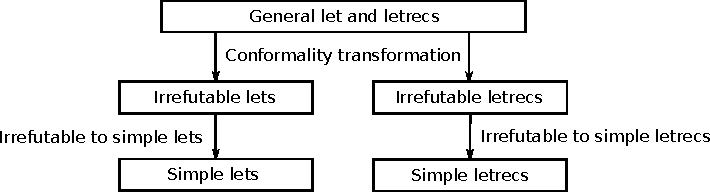
\includegraphics[height=4cm]{let_transform}
  \caption{Transformation of let(rec) expressions.}
  \label{fig:letrec_transform}
\end{figure}

\subsection{Refutable and irrefutable patterns.}
\label{sec:irrefutable_patterns}
We can distinguish two different types of let(rec) bindings: \textit{Refutable}
and \textit{irrefutable} ones. Lets look at this sample let expression:

\vspace*{0.2in}
\begin{lstlisting}[style=haskell,mathescape=true,label=lst:conformality_check,caption={Pattern matching let binding.}]
let (Cons x xs) = $expr$ in ...
\end{lstlisting}
The problem arises because \texttt{expr} might be evaluated to \texttt{Nil},
and in such situation this pattern matching will fail. This is precisely the
characteristic that distinguishes between the two aforementioned types of
let(rec) bindings. In short refutable bindings are those which contain
at least one refutable pattern and thus may fail during evaluation. On the
other hand irrefutable ones are those in which a failure cannot occur, thus
when all patterns are irrefutable.

\begin{definition}
  \label{def:irrefutable_pattern}
  A pattern is irrefutable if any of these conditions apply:
  \begin{itemize}
    \item It is a simple pattern (i.e. number pattern, character pattern, etc.)
    \item It is a variable pattern
    \item It has the form ($c$ $p_{1}$ $p_{2}$ \ldots $p_{n}$), where $c$ is
      constructor and $p_{1}$ $p_{2}$ \ldots $p_{n}$ are irrefutable patterns
  \end{itemize}
\end{definition}
The function \texttt{isRefutable} is implemented in exactly this fashion.

\subsection{Conformality transformation}
\label{sec:conformality_transformation}
A \textit{conformality transformation} is an activity to translate the program
into one that checks for patterns mismatch in let(rec) bindings. It
will contain only irrefutable let(rec) bindings. We say that such
program performs a \textit{conformality check}. Lets also mention that such
transformation is only needed in case of refutable bindings, so there is no need
to perform this, possibly expensive, computation in when patterns cannot fail.
So the first step of conformality transformation is partitioning
let(rec) bindings regarding to their refutability. Once we have all
patterns that might fail in one place we need to find a way to transform
let(rec)s into a form that conformality check is done.  Considering
our running example from Listing~\ref{lst:conformality_check} our compiler
would transform this expression into:

\vspace*{0.2in}
\begin{lstlisting}[style=haskell,mathescape=true]
let (Cons x xs) = let $v_{1}$ = $expr$
                  in (($\lambda$p.(Cons x xs)) $v_{1}$) [] Error
\end{lstlisting}
where $v_{1}$ is newly introduced unique variable.

Based on that observation we could derive the general form of conformality
transformation from:

\vspace*{0.2in}
\begin{lstlisting}[style=haskell,mathescape=true]
let $p_{1}$ = $e_{1}$;
    $p_{2}$ = $e_{2}$;
       $\vdots$
    $p_{n}$ = $e_{n}$
in $\ldots$
\end{lstlisting}
into:

\vspace*{0.2in}
\begin{lstlisting}[style=haskell,mathescape=true]
let
    ($c_{k1}$ $v_{1,1}$ $\ldots$ $v_{1,k1}$) = let $w_{1}$ = $e_{1}$
                      in (($\lambda p_{1}$.($c_{k1}$ $v_{1,1}$ $\ldots$ $v_{1,k1}$)) $w_{1}$) [] Error
                               $\vdots$
    ($c_{kn}$ $v_{n,1}$ $\ldots$ $v_{n,kn}$) = let $w_{n}$ = $e_{n}$
                      in (($\lambda p_{n}$.($c_{kn}$ $v_{n,1}$ $\ldots$ $v_{n,kn}$)) $w_{n}$) [] Error
in $\ldots$
\end{lstlisting}
where:
\begin{itemize}
  \item $c_{ki}$ is a constructor of arity equal to the number of variables
    bound by pattern $p_{i}$. Lets call the set of such variables $Var(p_{i})$
  \item $\{v_1, v_2, \ldots, v_n\} = Var(p_i)$
  \item $w_{i}$ is distinct from every $v \in Var(p_i)$
\end{itemize}
The function which calculates the $Var(p_i)$ set is called
\texttt{getPatternVarNames} and its behaviour is works by collecting already
seen variable names while recursively traversing the pattern:

\vspace*{0.2in}
\begin{lstlisting}[style=haskell]
getPatternVarNames :: Pattern -> [Name]
getPatternVarNames (PNum n) = []
getPatternVarNames (PChar c) = []
getPatternVarNames (PVar v) = [v]
getPatternVarNames (PConstr tag arity patterns) = foldl collectVars [] patterns
    where
        collectVars vars pattern = vars ++ getPatternVarNames pattern
\end{lstlisting}

The implementation of conformality transformation can be found in
\texttt{conformalityTransform} in \textit{LetTransformer.hs}.

\subsection{Transforming irrefutable lets into simple lets}
As previously mentioned irrefutable let is such that contain only
irrefutable patterns as binders. There are three cases in which we consider a
pattern irrefutable according to Definition~\ref{def:irrefutable_pattern}. In
the first two patterns on the left-had side of definition might be either
variable or simple patterns(numbers, characters, etc.). In such case these
patterns are already simple, so there is nothing else to do. On the other hand
when patterns are irrefutable constructor patterns they are take the following
form:

\vspace*{0.2in}
\begin{lstlisting}[style=haskell,mathescape=true]
  let ($c$ $p_1, p_2 \ldots, p_n$) = $expr$ in $\ldots$
\end{lstlisting}
where each $p_1, p_2, \ldots, p_n$ are irrefutable patterns. In order to
convert such expression into a simple let, we can apply the following
transformation\footnote{Without loss of generality we can assume that each
let contains only one definition. Every program could be easily
transformed to conform to this condition.}:

\vspace*{0.2in}
\begin{lstlisting}[style=haskell,mathescape=true]
let $v$ = $expr$
in (let $p_1$ = $Select\mbox{-}r\mbox{-}1$ $v$;
        $p_2$ = $Select\mbox{-}r\mbox{-}2$ $v$;
              $\vdots$
        $p_n$ = $Select\mbox{-}r\mbox{-}n$ $v$
    in $\ldots$)
\end{lstlisting}
Here, $v$ is a newly introduced variable, $r$ is the arity of the $c$
constructor, whereas each $Select\mbox{-}r\mbox{-}i$ is a function that selects
the $i^{th}$ component of a constructor with arity $r$. Again a simple example
should clarify this:

\vspace*{0.2in}
\begin{lstlisting}[style=haskell,mathescape=true]
let (Cons x xs) = (Cons 1 (Cons 2 (Cons 3 Nil)))
\end{lstlisting}
after applying the aforementioned transformation will be converted into:

\vspace*{0.2in}
\begin{lstlisting}[style=haskell,mathescape=true]
let $v$ = (Cons 1 (Cons 2 (Cons 3 Nil)))
in (let x  = $Select\mbox{-}2\mbox{-}1$ $v$;
        xs = $Select\mbox{-}2\mbox{-}2$ $v$)
\end{lstlisting}
$Select\mbox{-}2\mbox{-}1$ when applied to \texttt{(Cons 1 (Cons 2 (Cons 3
Nil)))} will yield \texttt{1}, and $Select\mbox{-}2\mbox{-}2$ is going to return
\texttt{Cons 2 (Cons 3 Nil)}.

\subsection{Transforming irrefutable letrecs into simple letrecs}
Transformation from irrefutable letrecs into simple ones is almost
identical to that concerning lets except from the fact that variables
from all definitions should be groupped together in order to ensure that
they are visible from other bindings. Here is the general scheme for such
conversion:

\vspace*{0.2in}
\begin{lstlisting}[style=haskell,mathescape=true]
letrec ($c_1$ $p_{1,1}, p_{1,2} \ldots, p_{1,n1}$) = $e_1$
       ($c_2$ $p_{2,1}, p_{2,2} \ldots, p_{2,n2}$) = $e_2$
                $\vdots$
       ($c_k$ $p_{k,1}, p_{k,2} \ldots, p_{k,nk}$) = $e_k$
in $expr$
\end{lstlisting}
is going to be translated into following expression:

\vspace*{0.2in}
\begin{lstlisting}[style=haskell,mathescape=true]
letrec
    $v_1$ = $e_1$;
    $p_{1,1}$ = $Select\mbox{-}n1\mbox{-}1$ $v_1$;
              $\vdots$
    $p_{n1,1}$ = $Select\mbox{-}n1\mbox{-}n1$ $v_1$;
    $v_2$ = $e_2$;
    $p_{2,1}$ = $Select\mbox{-}n2\mbox{-}1$ $v_2$;
              $\vdots$
    $p_{n2,1}$ = $Select\mbox{-}n2\mbox{-}n2$ $v_2$;
              $\vdots$
    $v_k$ = $e_k$;
    $p_{k,1}$ = $Select\mbox{-}nk\mbox{-}1$ $v_k$;
              $\vdots$
    $p_{nk,1}$ = $Select\mbox{-}nk\mbox{-}nk$ $v_k$;
in $expr$
\end{lstlisting}

\subsection{Summary}
After all these transformations took place, all binders in every
let(rec) expressions should become variable pattern in form
\texttt{PVar v = $expr$} or simple pattern. Now the pattern-matching algorithm,
described in Section~\ref{sec:pattern_matching_algorithm} can be used because
it was developed under assumption that left-hand sides of let(rec)
binders does not contain refutable and complex patterns. Therefore it is
important to run the conformality transform before pattern matching phase.

%\section{Transforming case expressions}

\section{Lambda Lifting}
\label{sec:lambda_lifting}
This section provides a description of how lambda abstractions are implemented
in Kivi. Lambda abstractions are more commonly known as \textit{local function}
or \textit{anonymous function} definitions concepts from imperative languages.
As previosly I am going to describe a program transformation, which when
applied, converts the program into a form where lambda abstracions become
global supercombinators. This transformation is known as \textit{lambda
lifting} or \textit{closure conversion}. The reader is encouraged to read the
Chapter 6 in \cite{JonLes00}, as well as Chapter 13 in \cite{Jon87} to
get additional information on this subject.

For the purpose of our \textit{lambda lifter} described here, I am going to
introduce the annotated version of Abstract Syntax Tree, that is capable of
carrying additional information needed for transformations described in this
chapter. The type that implements this was called \texttt{AnnExpr} and has
been placed in \textit{LambdaLifter.hs}. Its full definition is following:

\vspace*{0.2in}
\begin{lstlisting}[style=haskell,label=lst:annotated_expression]
type AnnExpr a b = (b, AnnExpr' a b)

data AnnExpr' a b = AVar Name
                  | ANum Int
                  | AChar Int
                  | AConstr Int Int
                  | AAp (AnnExpr a b) (AnnExpr a b)
                  | ALet IsRec [AnnDefn a b] (AnnExpr a b)
                  | ACase (AnnExpr a b) [AnnAlt a b]
                  | ACaseSimple (AnnExpr a b) [AnnAlt a b]
                  | ACaseConstr (AnnExpr a b) [AnnAlt a b]
                  | ALam [a] (AnnExpr a b)
                  | ASelect Int Int a
                  | AError String
    deriving Show

type AnnDefn a b = (a, AnnExpr a b)
type AnnAlt a b = (Int, AnnExpr a b)
data AnnScDefn a b = AnnScDefn Name [a] (AnnExpr a b)
type AnnProgram a b = [AnnScDefn a b]
\end{lstlisting}

As in the case for general \texttt{Expr} data type, each constructor is
responsible for creating a corresponding expression type. The \texttt{b} type
variable stands for additional information that the following passes will
produce. For instance, the \texttt{freeVars} pass described below, gathers the
free variables from the expression, so the \texttt{b} type will represent the
set of free variables in this expression. The full type in this case will have
the AnnExpr \texttt{AnnExpr Name (Set Name)} signature.

Lambda lifting is a way of eliminate free variables from local function
definitions. The elimination of free variables allows the compiler to hoist
lambda abstractions out of their surrounding contexts into a fixed set of
top-level supercombinators with extra parameter for each free variable. As an
example of this we will analyse the following Kivi function that multiplies two
integers without using the multiplication operator (in a rather not the most
optimal fashion)

\vspace*{0.2in}
\begin{lstlisting}[style=haskell]
mul 0 y = 0;
mul x 0 = 0;
mul 1 y = y;
mul x y =
    let sum a = y + a
    in sum (mul (x-1) y);
\end{lstlisting}

The \texttt{sum} lambda abstraction can be removed by introducting a new
\texttt{sum'} supercombinator, that takes an additional argument $t$ as shown at
the example below:

\vspace*{0.2in}
\begin{lstlisting}[style=haskell,mathescape=true]
$sum'$ $t$ a = $t$ + a
mul 0 y = 0;
mul x 0 = 0;
mul 1 y = y;
mul x y =
    $sum'$ y (mul (x-1) y);
\end{lstlisting}

Lambda lifter will define such supercombinator for each lambda abstraction and
each of these supercombinators will take additional arguments that has been
free in the body of lambda abstraction before transformation.

The lambda lifting algorithm consists of four parts executed one after another:

\vspace*{0.2in}
\begin{lstlisting}[style=haskell]
lambdaLift :: CoreProgram -> CoreProgram
lambdaLift (adts, scs) = (adts, collectScs . rename . abstract . freeVars $ scs)
\end{lstlisting}

I am going to describe and provide details of how each of them has been
implemented in Kivi. The source file to look for implementation details, is
\textit{LambdaLifter.hs}.

\subsection{Annotating expressions with free variables}
The first phase of an algorithm is to annotate each Abstract Syntax Tree
expression with free variable occurencs contained in it. As we can see in the
type signature for function \texttt{freeVars} it transforms a list of
supercombinator definitions into the similar list\footnote{\texttt{AnnProgram}
type, according to Listing~\ref{lst:annotated_expression}, is just the list of
annotated supercombinator definitions}:

\vspace*{0.2in}
\begin{lstlisting}[style=haskell]
freeVars :: [CoreScDefn] -> AnnProgram Name (Set Name)
\end{lstlisting}

More complicated code appears in the definition of function
\texttt{calcFreeVars} that has been called from \texttt{freeVars}. Its
arguments are:
\begin{itemize}
  \item \texttt{localVars} keeps variable names that has been defined in outer
    scopes. If, during traversing of AST such variable is used, it means that
    it s free variable of current expression.
  \item Expression to visit
\end{itemize}

The cases for simple expressions like \texttt{EVar} or \texttt{ENum} are easy,
the most complicated one occurs when calculating free vars for
let(rec) bindings. The code in this case works by calculating the free
variable set for each of the right-hand sides of bound variables. Then if it is
the recursive let, the free variable set consist of sum of these sets without
variables bound in current letrec binding. Otherwise it is simply the
sum of all free variables in right-hand sides.

\subsection{Abstracting free variables}
After each expression has the set of its free variables assigned, the algorithm
proceeds by abstracting out the free variables from each lambda abstraction and
introducting the let binding of the form:

\vspace*{0.2in}
\begin{lstlisting}[style=haskell,mathescape=true]
(let sc = \$v_1$ $v_2$ $\ldots$ $v_n$ $x_1$ $x_2$ $\ldots$ $x_n$ . $expr$ in sc) $v_1$ $v_2$ $\ldots$ $v_n$
\end{lstlisting}

for $v_1$, $v_2$, $\ldots$, $v_n$ being free variables of lambda abstraction.
The code responsible for this is in the \texttt{abstractExpr} function in the
branch where \texttt{ALam} expressions are considered:

\vspace*{0.2in}
\begin{lstlisting}[style=haskell]
abstractExpr (freeVars, ALam args expr) =
    foldl EAp sc $ map EVar freeVarsList
    where
        freeVarsList = Set.toList freeVars
        sc = ELet False [("sc", scBody)] (EVar "sc")
        scBody = ELam (freeVarsList ++ args) (abstractExpr expr)
\end{lstlisting}

The example of how this code would perform on a real case might be as the one
below. The lambda abstraction:

\vspace*{0.2in}
\begin{lstlisting}[style=haskell]
(\x . y * y + x * z + tmp)
\end{lstlisting}

will be transformed into:

\vspace*{0.2in}
\begin{lstlisting}[style=haskell]
(let sc = (\y z tmp x . y * y + x * z + tmp) in sc) y z x
\end{lstlisting}

\subsection{Renaming supercombinators}
The next step performs the renaming of variables, effectively giving unique
name to each of the \texttt{sc} variables introduced by let bindings
in previous step. Given that introduced supercombinators have unique names it
would be possible to hoist them to the level of global supercombinators during
next phases of algorithm. This is implemented as \texttt{rename} function. It
calls a generic renaming function \texttt{renameGen}. \texttt{renameGen} takes
as an input a function that generate new unique suffixes and concatenate them
with old variable names. It also requires that a list of supercombinator
definitions is given. It works by recursively visiting each AST expression and
performing a rename where applicable. Example function that is supposed to
rename variables in \texttt{EVar} expression:

\vspace*{0.2in}
\begin{lstlisting}[style=haskell]
renameExpr newNamesFun mapping ns (EVar v) =
    (ns, EVar v')
    where
        v' = case Map.lookup v mapping of
            (Just x) -> x
            Nothing -> v
\end{lstlisting}

Here, \texttt{mapping} is an instance of a \texttt{NameSupply} type. It is used
to carry around an information about already used names in form of map between
old variable name to new variable name. If currently considered variable is
already present in a map, it means that we should use the name saved there.

As a result \texttt{renameGen} and \texttt{rename} return supercombinators with
each variable name being unique.

\subsection{Collecting supercombinators}
Finally, in the last step, we can perform the 'lift part' of lambda lifting
algorithm. In this pass the supercombinators introduced earlier are collected
and raised to the top level.  Regarding source code, the only complicated bit
is in the \texttt{collectExpr} function when collecting supercombinators from
let(rec) expressions.  There are three possibilities where we should
collect supercombinators from:

\begin{itemize}
  \item Firstly, supercombinators might be nested in let(rec)
    expression. They are gathered by calling \texttt{collectExpr} on that
    expression and are stored in \texttt{exprScs} variable.
  \item Supercombinators might also be present directly as let(rec)
    bindings as $sc$ \texttt{=} $\lambda v_1$ $\ldots$ $v_n$ . $expr$.
    Therefore what Kivi does, is splitting the list of bindings into ones that
    are simple variable bindings and supercombinators.
  \item The third and the last possibility is when supercombinators are nested
    in the right-hand side of binding. Then we should extract them by means of
    calling the \texttt{collectExpr} on the right-hand side of binding
    definition. This is implemented by folding over bindings with
    \texttt{collectDef}.
\end{itemize}

\section{Full laziness}
\textit{Full laziness} refers to the optimization technique used in functional
languages, that makes calculation of value of each expression in a computer
program to occur at most once. A similar mechanism is used to in imperative
language compilers when optimizing loops. Expressions that cannot change during
loop's execution(\textit{loop invariants}) are moved outside a loop in order to
prevent it from being recalculated multiple times.
\textit{Lazy lambda lifting} is an optimization of lambda lifting technique to
ensure full laziness. Ordinary lambda lifter used to make each free variable of
a lambda abstraction a parameter to the new supercombinator. Lazy lambda lifter
makes one step ahead and isolates \textit{maximally free subexpressions}
(further referred as \textit{MFE}s) which are later used as supercombinator
arguments instead. For that reason MFEs will be shared so their value will be
calculated at most once. MFE is defined as follows:

\begin{definition}
  Maximally free subexpression e of a lambda abstraction is a maximal
  expression holding two properties:

  \begin{itemize}
    \item it does not contain variables bound by that lambda abstraction.
    \item e is not a subexpression of larger expression containing occurences of
      variables bound by lambda abstraction
  \end{itemize}
\end{definition}

As an example of how it works, consider the following Kivi function:

\vspace*{0.2in}
\begin{lstlisting}[style=haskell]
f y =
    let g = (\x . x + y * y)
    in (g 1) + (g 2)
\end{lstlisting}

Simple lambda lifter described in Section~\ref{sec:lambda_lifting}, will
calculate the \texttt{y * y} expression twice each time \texttt{f} is called.
Transformation desribed above will identify \texttt{y * y} as MFE and make it
an argument of a newly created supercombinator \texttt{g}. Thus, after this
step, the expression will be transformed to following one, making the \texttt{y
* y} to be calculated once per each call of \texttt{f}:

\vspace*{0.2in}
\begin{lstlisting}[style=haskell,mathescape=true]
g v x = x + v
f y = let $v$ = y * y
      in (g $v$ 1) + (g $v$ 2)
\end{lstlisting}

\subsection{Handling let(rec)s}
This above approach works perfectly well until one realizes that let(rec)
expressions cannot be handled this way. The problem is illustrated in listing
below:

\vspace*{0.2in}
\begin{lstlisting}[style=haskell]
f x = let g = (\y . let a = x * 2
                    in let b = a + 1
                    in b + y)
      in g 1 + g 2
\end{lstlisting}

In construct shown below, the above algorithm will not be able to deduce that
expression for \texttt{b} depends only on \texttt{x}, because it directly
depends on \texttt{a} which was bound inside \texttt{g} lambda abstraction.
This will result in value for expression \texttt{b} being calculated twice for
each call to \texttt{f}. Nevertheless a full laziness requires this value to
be calculated at most once.

Simple fix that allows let(rec)s to be handled correctly consist of
\textit{floating} them as far as possible, in our case yielding the following
program:

\vspace*{0.2in}
\begin{lstlisting}[style=haskell]
f x = let g = let a = x * 2
              in let b = a + 1
              in (\y . b + y)
      in g 1 + g 2
\end{lstlisting}

In order to determine how far each let(rec) should be floated, the \textit{free
variable set} needs to be calculated for each let(rec) bound variable.

\begin{definition}
  Free variable set of variable x is the set of free variables
  that x depend on. Free variable set for let(rec) is the sum of free
  variable sets of all let(rec) binders.
\end{definition}

Each let(rec) should be floated until the next surrounding lambda abstraction
binds any of variables in let(rec)'s free variable set. This is implemented by
assigning level numbers to each let(rec)-bound variable, as well as for each
variable defined by lambda abstraction. Level number for a let(rec) bound
variable $v$, is a maximum of levels of free variables occuring in definition
of $v$. On the other hand, level number of a variable $v$ introduced by lambda
abstraction is the number of lambdas that surrounds $v$. By comparing these
values during AST traversal, the algorithm knows which let(rec) bindings are to
to be floated outwards.

\subsection{Handling MFEs}
There is another simple transformation that allows MFEs to be handled by
algorithm described for let(rec)s. It consists of substituting every expression
$e$ that is a maximally free subexpression of any enclosing lambda, for
expression \texttt{let $v$ = $e$ in $v$}, where $v$ is a newly introduced,
unique variable. Let bindinges created in this way will become available for
let(rec) lifter described above, so it's important to execute this
transformation before floating part.

Logic described in this section is possible to be implemented in a separate
pass, instead of modifying the basic lambda lifting algorithm, and this is the
approach I have taken.

\subsection{Implementation}
Implementation of lazy lambda lifter is contained in
\textit{LazyLambdaLifter.hs} file. It consists of six passes that are going to
bescribed below, starting from innermost one, and is implemented as function
\texttt{lazyLambdaLift}:

\vspace*{0.2in}
\begin{lstlisting}[style=haskell]
lazyLambdaLift :: CoreProgram -> CoreProgram
lazyLambdaLift (adts, scs) =
    (adts, float
         . mergeLambdas
         . renameL
         . identifyMFEs
         . annotateLevels
         . separateLambdas $ scs)
\end{lstlisting}

\subsubsection{Separating lambdas}
The first part is executed in order to separate each lambda abstraction in a
way that it contains only one argument. This behaviour is imlemented as
\texttt{separateLambdas} function. When it encounters a lambda abstraction, we
fold over the arguments and for each of them create a separate lambda that
binds a single argument only.

\subsubsection{Calculating levels}
For the purpose of calculating the levels of expressions and binders it is
necessary to first annotate each expression with free variables that occurs in
it. This can be done by reusing the \texttt{freeVars} function defined earlier
for a regular lambda lifter in Section~\ref{sec:lambda_lifting}. Once it is
done, level of each lambda or let bound variable $v$ can be calculated by
finding the innermost lambda that binds any of $v$'s free variables. The
\texttt{annotateLevels} function works in exactly this way and returns an
instance of \texttt{AnnProgram (Name, Level) Level} type. As we recall the
\texttt{AnnExpr} definition from Section~\ref{sec:lambda_lifting}, it means
that each binder and each expression are now associated the appropriate levels:

\vspace*{0.2in}
\begin{lstlisting}[style=haskell]
annotateLevels :: [CoreScDefn] -> AnnProgram (Name, Level) Level
annotateLevels = freeToLevel . freeVars
\end{lstlisting}

First interesting case arises when analysing lambda abstractions. Level of
lambda abstraction is calculated by \texttt{freeSetToLevel} that takes a
mapping between names and levels as well as free variables set and returns the
maximum of levels of all variables in the set:

\vspace*{0.2in}
\begin{lstlisting}[style=haskell]
freeSetToLevel :: Map Name Level -> Set Name -> Level
freeSetToLevel env free =
    maximum [ case Map.lookup var env of
        Just level -> level
        Nothing -> 0 | var <- (Set.toList free)]
\end{lstlisting}

Because each lambda-bound variable's level is the number of lambdas enclosing
it, we can simply set it to the level of its context incremented by one.

Another case that demands more care arises when calculating the levels of
let(rec) bindings. Here, the level of let(rec) is set to level of let(rec)'s
body, and levels of binders are assigned a maximum of levels of free variables
occuring on right-hand-side of any binder.

\subsubsection{Identifying MFEs}
Next phase consists of identification and transformation of found MFEs.
Implementation is rather straightforward. Function \texttt{identifyMFEsExpr}
compares the levels of enclosing context with level of current expression. If
they differ it means that we have found an MFE. After this check, function is
recursively applied to subexpressions. One thing to be mentioned however, is
the fact that there is no need to mark simple expressions, such as variables or
constant values, as MFEs in order to avoid clutter.

\subsubsection{Renaming variables}
Rename pass takes place after identifying MFEs to rename all binders. This
part is neccessary in order to avoid errors that can be caused during floating
because of duplicate identifiers present. It exploits the generic function
\texttt{renameGen} used earlier in lambda lifting (see
Section~\ref{sec:lambda_lifting}).

\subsubsection{Merging lambda abstractions}
This phase is the opposite of separating lambda abstractions performed at the
beginning. Here we merge the directly nested lambda abstractions into one that
binds all the arguments.

\subsubsection{Floating let(rec)s}
The final pass lifts let(rec)s to appropriate levels. Each expression is
annotated with \texttt{FloatedDefns} type:

\vspace*{0.2in}
\begin{lstlisting}[style=haskell]
type FloatedDefns = [(Level, IsRec, [(Name, Expr Name)])]
\end{lstlisting}

It is the list that contains bindings to be floated outwards along with its
level. The most interesting cases again occur for lambdas and let(rec)s.

When floating lambda abstractions, definitions floated from inside of lambda's
definition are partitioned according to their level. Those with level with
value less that lambda's one, are lifted further, whereas others are placed
inside lambda, by defining an appropriate let construct (see \texttt{wrap}
function in listing below). The code performing the above logic is presented
below:

\vspace*{0.2in}
\begin{lstlisting}[style=haskell]
floatExpr (ELam args expr) = (outerFds, ELam args' $ wrap innerFds expr')
    where
        args' = [arg | (arg, level) <- args]
        (_, curLevel) = head args
        (fdBody, expr') = floatExpr expr
        (innerFds, outerFds) = List.partition checkLevel fdBody

        -- predicate to partition the definitions based on definition level
        checkLevel (level, isRec, defns) = level >= curLevel

        -- helper function which wraps an expr into let binding with given defns
        wrap floatedDefns expr =
            foldr wrapDefn expr floatedDefns
            where
                wrapDefn (level, isRec, defns) expr = ELet isRec defns expr
\end{lstlisting}

In let(rec) case, there are three sources of floated definitions. First two are
extracted from binder right-hand-sides and let(rec) body. The last one consists
of local definitions introduced by let(rec) itself. These all, are combined into
single list and floated outwards until the next lambda abstraction.

\section{Dependency Analysis}
Dependency analysis is a process of splitting up let(rec) bindings
into minimial-sized groups and preferring let over letrec
where possible. The reason for this choice is because the non-recursive version
of binding can be implemented more efficiently. The fact that let(rec)
expressions are not always as optimal as they could, is twofold:
\begin{itemize}
  \item First, programmer might have ommited the fact that the
    let(rec) expression he implemented is not recursive at all.
  \item Previous phases\footnote{as well as passes that are not yet available
    in Kivi} might be unnecesarily pessimistic, for example where
    clauses are always transformed into recursive lets for simplicity
    reasons.
\end{itemize}
Consider the following Kivi binding as an illustration of that fact:

\vspace*{0.2in}
\begin{lstlisting}[style=haskell,label=lst:letrec_dependency_example,caption={Example of
  letrec before dependency analysis.}]
letrec
    p       = res + 1;
    q       = res + 2;
    x       = p + q;
    fac n   = if (n == 0) 1 (n * fac(n-1));
    res     = fac x;
    gcd a b = if (b == 0) a (gcd b (a % b))
in
    gcd res 3
\end{lstlisting}
After analysing the dependencies and splitting the letrec into minimal
subgroups the expression will become:

\vspace*{0.2in}
\begin{lstlisting}[style=haskell,label=lst:letrec_after_anlysis,caption={letrec
  after performing dependency anlysis.}]
letrec
    fac n = if (n == 0) 1 (n * fac(n-1))
in letrec
    gcd a b = if (b == 0) a (gcd b (a % b))
in letrec
    p = res + 1
    q = res + 2
    x = p + q
    res = fac x
in
    gcd res 3
\end{lstlisting}
This section provides an efficient algorithm to perform dependency analysis
using \textit{strongly connected components}.

\subsection{The Algorithm}
The algorithm consists of a few steps that will be described below. The source
code for this logic has been placed in \textit{DependencyAnalyser.hs} module
with \texttt{analyseDeps} function as an entry point. However in order to fully
understand further deliberations, it is necessary to introduce a couple of
definitions, that will be given througout this section.
\begin{definition}
A directed graph is a pair G = (V, E) of:
\begin{itemize}
  \item a set V, whose elementes are called vertices or nodes,
  \item a set E of ordered pairs of vertices, called arcs, directed edges, or
    simply edges.
\end{itemize}
\end{definition}

\subsubsection{Constructing Dependency Graph}
The first step of dependency analysis algorithm is to create a
\textit{dependency graph} for each each letrec construct. It is
defined as follows:
\begin{definition}
A dependency graph is a directed graph, where:
\begin{itemize}
  \item a set $V$ of vertices is the set of all variables bound by
    letrec
  \item there is an edge from vertex representing variable a to vertex
    representing variable b, if b is present in the right-hand side of
    binding for a. Formally speaking, if b occurs as a free variable
    (Definition~\ref{def:free_variable}) definition of a.
\end{itemize}
\end{definition}

To get a feeling how this applies in practice lets look at the dependency graph
build for our example from Listing~\ref{lst:letrec_dependency_example}:

\vspace*{0.2in}
\begin{figure}[h!]
  \centering
  \includegraphics[height=4cm]{dependency_graph}
  \caption{Dependency graph constructed for letrec binding.}
  \label{fig:letrec_dependency_graph}
\end{figure}

\subsubsection{Strongly Connected Components}
Next in order to group variables that depend on each other into one letrec
binding, we have to determine which variables are mutually recursive. This is
done by calculating the \textit{strongly connected components} (or
\textit{SCC}) of a dependency graph. To gain a deep insight into analysis of an
algorithm, see \cite{Cormen03}. Definition of strongly connected components can
be found below:

\begin{definition}
Directed graph is said to be strongly connected if there is a path from each
vertex in the graph to every other vertex. In particular, this means paths in
each direction: a path from a to b and also a path from b to a.
The strongly connected components of a directed graph G are its maximal
strongly connected subgraphs.
\end{definition}

Strongly connected components found for dependency graph formed for running
example is presented in Figure~\ref{fig:topsorted_scc}. There will be three
coalesced vertices created and they are shown by dotted lines.

\vspace*{0.2in}
\begin{figure}[h!]
  \centering
  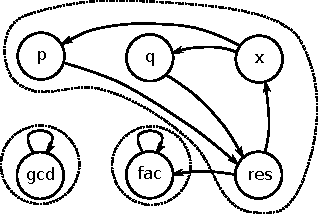
\includegraphics[height=5cm]{scc_graph}
  \caption{Strongly connected components of a dependency graph.}
  \label{fig:topsorted_scc}
\end{figure}

\subsubsection{Topological Sorting}
After successfully determining the maximal sets of mutually dependent variable
bindings, it is time to find out which of these groups depend on each other.
Exploiting this information will make it possible to arrange bindings in letrec
in a way that all needed variables will be in scope when evaluating the value
of bindings that depend on them. The way to perform this step is to transform
the graph further by coalescing each strongly connected component into a single
vertex.  The resulting graph will be acyclic, so it would become possible to
sort the coalesced vertices \textit{topologically}. Again the full description
of \textit{topological sorting} algorithm can be found in \cite{Cormen03}.

\subsubsection{Building a new letrec}
The last step is to create the letrec binding for each strongly
connected component in topological order. In our example the structure from
Listing~\ref{lst:letrec_after_anlysis} will be created.


\subsection{Implementation}
Regarding implementation issues, the heart of the code responsible for
aforementioned tasks is implemented in \texttt{analyseExpr} function in case
for let(rec) expressions. First of all, each AST expression is
augumented with its free variables. Based on that, function \texttt{getEdges}
folds over letrec bindings and creates edges of the dependency graph:

\vspace*{0.2in}
\begin{lstlisting}[style=haskell]
getEdges edges (name, (rhsFree, rhs)) =
    edges ++ [(name, v) | v <- (Set.toList $ Set.intersection binderSet rhsFree)]
\end{lstlisting}

Next, \texttt{scc} function is invoked in order to find strongly connected
components of dependency graph. It does so by first computing, for each vertex
$x$, the set of vertices accessible (directly or indirectly) from that vertex
using forward edges, as well as sets of vertices accessible using backward
edges. By computing the intersection of these sets, we can effectively get
component of vertex $x$:

\vspace*{0.2in}
\begin{lstlisting}[style=haskell]
scc :: Show a => Ord a => (a -> [a]) -> (a -> [a]) -> [a] -> [Set a]
scc ins outs vs = topSortedSccs
    where
        topSortedVs = snd $ dfs outs (Set.empty, []) vs
        topSortedSccs = snd $ spanDfs ins (Set.empty, []) topSortedVs
\end{lstlisting}

The rest of the \texttt{analyseExpr} function is meant to split the input
letrec expression according to the computed strongly connected
component set.

\chapter{Type checking}
\textit{Type checking} is a process verifying and demanding certain conditions
to hold in regard to types of objects in a computer program. One way to
categorize programming languages is by the time when type checking is
performed. There are two major notions of how it can be implemented in modern
programming languages. The process of checking and enforcing constraings on
types can take place either at compile-time, which is often called a
\textit{static typing} or during run-time, which is known as \textit{dynamic
typing}.

\section{Static and Dynamic Typing}
Static typing allows to catch many type errors early in the development cycle.
This, at least in theory, should improve the robustness of the final program.
Nevertheless that static type checker can only utilize information that are
present during compile-time, it can prove that checked conditions will hold for
every possible execution path of a progrem. This successfully eliminates the
need to perform type checking for every execution of a program, as will be the
case in dynamically typed languages. It might result in faster execution times
and more optimal memory usage.

On the other hand, languages that are dynamically typed, are those in which
type checking is performed during run-time instead of compile-time. Internally,
type information is gathered in form of tags that are then associated with
objects and contain, among other data, information about types. Variables in
dynamically typed languages can refer to data of any type, so variables does
not have a type, whereas data does. Dynamic languages does not enforce as high
level of conservativeness as static ones, which may result in run-time errors.
However the lack of compile-time checks may result in faster compilation times
and easier adoption of dynamic programming language features thans to data
available at runtime. This data might also make it possible to perform more
advanced type checks which might result in certain optimizations which would
otherwise be impossible.

\section{Polymorphism}
Polymorphism, in regard to programming languages, relates to the ability of a
computer program to contain many types or to act on many types. The common way
to achieve it is to allow different instances of certain structures to perform
operations on different types of data. This way it will allow the same code to
be executed on different kinds of objects, thus allowing a programmer to
effectively reuse code. There are few different kinds of polymorphism, but the
one that I will be particularly interested in is called \textit{parametric
polymorphism} \cite{Car88}.

Parametric polymorphism is a language feature that allows one piece of code to
act in the same way on chunks of data that may not necessarily have the
identical type. In this context word \textit{parametric}, refers to types of
objects, which may be seen as \textit{parameters} of some block of code. There is a
distinction between two kinds of parametric polymorphism:

\begin{itemize}
  \item \textit{explicit parametric polymorphism} is one in which types of
    variables and function arguments are given explicitly in the code by the
    programmer.
  \item \textit{implicit parametric polymorphism} on the other hand, occurs
    when type declarations are not present directly in source and types can
    contain type variables, which are \textit{holes} to be later filled with certain
    types.
\end{itemize}

In case of implicit polymorphism, information that has been omitted have to
later be rediscovered. The ability of a compiler to deduce missing types
(either fully or partially) is called \textit{type inference}. Using a compiler
that supports implicit polymorphism, as well as has inferencing mechanisms
implemented, a programmer can leave out the types of expressions while having
his program rigorously type-checked as the types were there. It has to be
mentioned however, that can be successfully typed using explicit polymorphism,
but types cannot be inferred for them using implicit one.

The algorithm to type check the program, that I have implemented in Kivi, is
known as \textit{Hindley-Milner algorithm}. Its most appealing property is that
type inference comes at no extra cost. In its search for missing types, the
most general typing possible is returned.

\section{Hindley-Milner algorithm}
Informally Hindley-Milner algorithm works by inspecting an expression and
creating a set of type constraints that are based on the usages of certain
values. Once the set is complete, the process called \textit{unification} takes
place in order to reconstruct the types. Unification checks whether there exist
a typing, such that all constraints would be satisfied. In case such typing
exist, it means that expression is well-typed and the typing is returned.
On the other hand if at least two constraints cannot be unified to a common
type, it means that algorithm is incapable of devising a correct typing for an
expression. As an example consider the following function
definition\footnote{The case when \texttt{head} is given an empty list is
ommitted in order to reduce verbosity.}:

\vspace*{0.2in}
\begin{lstlisting}[style=haskell]
head (x : xs) = x
\end{lstlisting}

First step is to assign fresh type variable to every function parameter as
well as its return type. This serves as initial set of constraints:

\vspace*{0.2in}
\begin{lstlisting}[mathescape=true,style=haskell]
  x :: $\alpha$
  xs :: $\beta$
  head :: $\gamma \rightarrow \delta$
\end{lstlisting}

From the set of built-in constraints we know that \texttt{:} is a cons operator
of type $\epsilon \rightarrow [\epsilon]$ so we can unify $\gamma$ to
$[\epsilon]$. Therefore we know that \texttt{head} takes list as an argument.
Also because of that we can unify $\alpha$ and $\beta$, the types for
\texttt{x} and \texttt{xs} variables, with respectively $\epsilon$ and
$[\epsilon]$:

\vspace*{0.2in}
\begin{lstlisting}[mathescape=true,style=haskell]
  x :: $\epsilon$
  xs :: $[\epsilon]$
  head :: $[\epsilon] \rightarrow \epsilon$
\end{lstlisting}

This completes the derivation of types for \texttt{head} function. It was an
informal look of how Hindley-Milner retrieves missing types. In order to gain
more insight of how real algorithm works, I encourage to read the rest of this
chapter which dives into the implementation details.

\subsection{Implementation}
Implementation of Hindley-Milner type checking algorithm can be found in
\textit{TypeChecker.hs} module. One of the first things that is defined in this
file is the data type to represent types itself. Types can be either type
variables or type operators. Type variables are created using \texttt{TypeVar}
constructor and consist of name as well as an instance which could be either be
null, or represent another type variable (creating a recursive chain) or a type
operator. \texttt{TypeOp} creates type operators. A type operator might
be either simple, such as \texttt{int} or \texttt{bool} or complex. As en
example of complex type operator consider the $\rightarrow$, presented
above, standing for function types. Complex type operators take other types as
arguments.

\vspace*{0.2in}
\begin{lstlisting}
data TypeExpr = TypeVar TypeVarName (Maybe TypeExpr)
              | TypeOp String [TypeExpr]
\end{lstlisting}

Type checking process can be summarized as matching type operators and
instantiating type variables. Occurences of the same variables depend on each
other. That means that whenever type variable $\alpha$ is instantiated to some
type, every other occurence of $\alpha$ must be instantiated to the same type
too. This process is known as \textit{unification}. During algorithm execution
information about instances is present in the \texttt{typeInstanceEnv}
component of a \texttt{State}. \texttt{State} contains also a \texttt{typeEnv}.
It is a simple mapping between names of variables and types representing these
variables. The last piece of state is a set of \textit{non-generic} type
variables:

\begin{definition}
  A type variable v occuring in the body of expression e is generic within this
  expression, if and only if it does not occur in the type of the binder of any
  lambda abstraction enclosing e.
\end{definition}

The above definition means that different occurrences of a generic type
variable in a type expression may be instantiated to different types. It can be
implemented by simply performing a deep-copy of the type variables and making
the non-generic ones shared between instances. In order to determine whether
the variable is generic during run-time of an algorithm, we can just check if
\texttt{nonGeneric} set contains it.

\subsubsection{Supercombinators}
Type checking is performed for each supercombinator. First each variable
introduced in supercombinator arguments is assigned a new and unique type
variable. The actual type of this variable is to be deremined later by its
occurences in supercombinator body. The mapping between argument name and its
type variable is saved in \texttt{typeInstanceEnv} variable. In order to do
this the body of a supercombinator is type-checked and returned type is
considered to be the type of supercombinator. This logic is implemented by
\texttt{typeCheckSc} function.

\subsubsection{Applications}
When \texttt{typeCheckExpr} enounters an application type of expression, the
type-checking is performed for both function and argument part of application.
New type variable is created for function result type. Assume that type
inferred for function argument is $t_a$, for function is $t_f$ and for result
$t_r$, then the algorithm has to unify type $t_a \rightarrow
t_r$ with $t_f$. This implies that the type for $t_f$ is indeed a function
type\footnote{because $\rightarrow$ operator represents function types} whose
domain is $t_a$ and the codomain is type of result, $t_r$.

\subsubsection{Let(rec) bindings}
In order to type-check let expressions, first type-checking of
bindings introduced by let takes place, obtaining an updated
environment, \texttt{typeInstanceEnv}. Body of let will by checked
using this fresh environment. The situation changes a bit in case of recursive
let expressions. Before analysing each definition it is necessary to
first assign a new type variable to each bound variable, creating an updated
environment. Once the new environment is available, types are checked for each
definition body as well as the body of a whole letrec in the end.

\subsubsection{Lambda abstractions}
There is no need to typecheck anonymous functions, as the lambda lifter
translated them to a top-level supercombinators.

\subsubsection{Identifiers and Constants}
In case of identifiers a \textit{fresh type} needs to be retrieved. Non-generic
type variables are shared between fresh and old type, whereas generic ones are
copied. Type-checking constants are straight-forward because an algorihtm
immediately knows its type. Therefore, for ints the \texttt{int} type operator
is returned, for booleans the \texttt{char}, etc.

\chapter{The G-machine}
The G-machine is an implementation of virtual machine based on the idea of
\textit{graph reduction} that will be described in
Section~\ref{sec:graph_reduction}. It works by compiling supercombinators into
intermediate code called \textit{G-code} and later translating it further or
executing in an interpreter.

The advantage of choosing the intermediate representation instead of compiling
to a particular machine code lies in a fact that it would require rewriting of
the whole compiler if later decided to change the machine. Moreover, one of the
main characteristics of intermediate representations is the fact that they
should resemble the original source language, and generating the machine code
from it, should remain simple as well. Thus, translating the original source
code first into the G-code and later to the machine of our choice shall be much
simpler than doing it in a straight-forward manner. The third argument for
preferring having intermediate representation over a concrete one is that it
will give us the ability to create virtual machine interpreters or compilers
for any particular computer architecture we desire, by means of only switching
the code generator. Code generators will then need to transform the
intermediate language into machine code of that machine. This will greatly
simplify the development of such tools, because the issues of compiling
supercombinators to sequential code and compiling to machine code will be
clearly separated.  Thanks to these facts I was able to easily create two
implementations of the G-machine:

\begin{itemize}
  \item The first one, is a G-machine interpreter. It is particularly suited
    for debugging purposes and it might be used as a Kivi shell in future. It
    was created in Haskell, and described in Section~\ref{sec:interpreter}
  \item Another one generates the intermediate code for Low Level Virtual
    Machine, which later is compiled to machine code by LLVM compilers. Its
    description is the content of Section~\ref{sec:llvm_codegen}.
\end{itemize}

\section{Graph reduction}
\label{sec:graph_reduction}
As previously stated the output of a syntax analyser is an Abstract Syntax
Tree. In above chapters we have applied a several transformations the the tree
so as to either allow special constructs like lambda abstractions or to
translate the source of the program to enriched lambda calculus. Eventually the
output of these transformations is still AST. \textit{Graph reduction} is an
implementation of efficient, non-strict supercombinator evaluation strategy.
Non-strictness in this context means that function arguments are evaluated on
demand. This is also known as \textit{lazy evaluation}. Another feature of
G-machine implementation is that values should only be evaluated once, in order
not to repeat the same calculations over and over.

\subsection{The Graph}
The abstract syntax tree is transformed to a graph due to conversions that take
place during graph reduction. Such graph is being stored in memory,
specifically it is kept on the heap. The nodes of the graph are dynamically
allocated on the heap. They contain a \textit{tag} that uniquely identifies the
type of a node, as well as additinoal fields like values, in case of number
nodes, or links (addresses) to other nodes in case of application nodes for
instance. For example the abstract way of visualising application and number
nodes might be like in the figure~\ref{fig:num_ap_nodes}:

\vspace*{0.2in}
\begin{figure}[h!]
  \centering
  \includegraphics[height=3cm]{nodes}
  \caption{Application and number nodes on the heap.}
  \label{fig:num_ap_nodes}
\end{figure}

\subsection{Evaluation Strategy}
There are many possible evaluation strategies. Many imperative languages
chooses to follow the \textit{innermost evaluation}. In this strategy the
arguments to a function are evaluated before the function application. In Kivi,
similarly as in other lazy functional languages the outermost redex is
evaluated first, thus Kivi adapts the \textit{innermost evaluation strategy}.
Function arguments are evaluated only in case it is absolutely needed, so
function arguments that are not used in the body of function will never be
evaluated, thus saving computations.

In Kivi reduction starts by evaluating the body of \texttt{main}
supercombinator. The process of reduction consist of transforming a graph
according to the specified rules and eventually arriving to the state where it
cannot be reduced any more. Such state is called \textit{weak head normal form}
(or WHNF for short). We assume that an expression is in the WHNF in several
cases. First of all, when it is a number, character, or any other simple data
type it is considered to be in WHNF. Another situation where there is nothing
more to reduce is if the expression is in ($f$ $e_1$ $e_2$ $\ldots$ $e_n$)
form, where $f$ is lambda abstraction, built-in function or constructor and $n$
is less or equal the expected number of arguments for $f$.

The process of evaluation can be described in four points:

\begin{itemize}
  \item Finding the next reducible redex
  \item If there is no redex which can be evaluated, then stop
  \item Otherwise reduce the redex
  \item Update the root of the redex, to save the result of computations
\end{itemize}

\subsection{Finding next redex}
The first step is to find the node of a graph where to perform the next
reduction. As already mentioned, among all such nodes we will be looking for the
outermost one. The most straight-forward way to find it, is to follow the left
branches of application nodes (as shown in Figure~\ref{fig:application_node})
saving the traversed node addresses on the runtime stack. There are two cases
when this process stops, either when the supercombinator or built-in function
node is encountered.

\subsection{Reduction}
Reduction depends on the type of node the algorithm encountered. There are a
few cases that might occur:

\subsubsection{Reducing supercombinators}
When supercombinator node is to be reducted, first thing what G-machine does,
is to check whether there are enough arguments on the stack. If it is not the
case, algorithm returns, as such application appears to be a \textit{partial
application} forming a closure. On the other hand, if the number of arguments
on the stack is greater or equal to the expected number the process continues.
The arguments to a supercombinator consist of a set of right children of
application nodes that we have visited during traversal\footnote{At this step,
the \textit{rearrangement} of arguments takes place. This activity will be
described in next chapters, but it is just an optimization so I am not going to
introduce it right now, not to make unnecessary complications.}. The addresses
that form the stack, are called \textit{spine} of the expression, and the
process of following the left branches of application nodes is commonly known
as \textit{unwinding} the spine. The reduction of a supercombinator can be
looked at, as instantiating a supercombinator body with arguments substituted
for formal parameters (as defined in Section 2.1.4 of \cite{JonLes00}).

\subsubsection{Reducing built-ins}
It might be the case however that the outermost redex found is not a
supercombinator node, but rather a built-in operator or function. In such case,
before applying the builtin, the required arguments should be evaluated to
WHNF. Therefore when evaluator finds itself in a state when built-in function
is the currently encountered node, it has to save the current stack on the
\textit{dump} and recursively invoke itself on all arguments that are not in
WHNF. Of course it might happen that during evaluation of arguments, the
algorithm once again runs into a situation when another builtin is to be
evaluated. In such case, it saves the current stack again and performs another
recursive invokation of itself. Dump therefore, is formed by putting stacks on
each other, so it might be perceived as stack of stacks.

This situation described above occurs when evaluating the expression \texttt{(1
+ (sqr 2)) * 3}. The graph built for this expression will look like one in
Figure~\ref{fig:expression_graph}, where inner nodes represented by black
circles are application nodes.

\vspace*{0.2in}
\begin{figure}[h!]
  \centering
  \includegraphics[height=7cm]{gmachine_graph}
  \caption{Graph created for expression \texttt{(1 + (sqr 2)) * 3}.}
  \label{fig:expression_graph}
\end{figure}

Because \texttt{*} operator is a builtin, it requires that all its arguments
are in WHNF before being able to continue. The algorithm puts the current stack
onto a dump and starts to evaluate the first argument. Shortly it will run into
a state that \texttt{+} is to be applied, but once again \texttt{sqr 2} is not
in a WHNF, so the process continues.

\subsection{Updating}
\label{sec:updating}
When reduction is complete, there is a need to save results of our
computations. This is called \textit{updating} the root of redex. Important
thing to notice is that if the redex is shared between two nodes of our graph,
the evaluation should be done only once. In order to achieve this we have to
introduce a new node type called \textit{indirection node}. Otherwise the
reduced node (result of computations) will have to be copied to the root of
the redex. In case of that node not being fully evaluated it brings a risk of
performing computations multiple times. Indirection nodes work like a pointer
to other node, effectively making the machine to use the values computed last
time redex was reduced. This will prevent it from performing the same
calculations more than once.

\subsection{Evaluation Example}
Example of evaluating expression (TODO: example expression) is presented
in Figure~\ref{fig:example_reduction}.

\begin{figure}[h!]
  \centering

  TODO: Obrazek ilustrujacy stos i zbudowane w ten sposob drzewo ewaluacji
  wyrazenia

  \caption{Example reduction process.}
  \label{fig:example_reduction}
\end{figure}

\section{Compiling supercombinators}
Compilation is a process of turning supercombinator body into a sequence of
G-machine instructions. These instructions when executed will construct an
instance of a supercombinator with formal parameters substituted with actual
function arguments. When running a concrete program, consisting of
supercombinator definitions, at first it will be translated into G-code, and this
process may be seen as \textit{compile time}. Later G-code is going to be
executed on a virtual machine, the G-machine. The latter may be regarded as
\textit{run time}.


\subsection{Instruction set}
In Kivi the set of G-code instructions available is presented as an excerpt
from \textit{Common.hs} module below:

\vspace*{0.2in}
\begin{lstlisting}[style=haskell]
type GmCode = [Instruction]

data Instruction = Unwind
                 | Pushglobal Name
                 | Pushconstr Int Int
                 | Pushint Int
                 | Pushchar Int
                 | Push Int
                 | Mkap
                 | Update Int
                 | Pop Int
                 | Slide Int
                 | Alloc Int
                 | Eval
                 | Add | Sub | Mul | Div | Neg | Mod
                 | Eq | Ne | Lt | Le | Gt | Ge
                 | Pack Int Int
                 | CasejumpSimple (Assoc Int GmCode)
                 | CasejumpConstr (Assoc Int GmCode)
                 | Select Int Int
                 | Error String
                 | Split Int
                 | Print
                 | Pushbasic Int
                 | MkBool
                 | MkInt
                 | Get
\end{lstlisting}

Here, \texttt{GmCode} type represents the G-code and is a simple list containing
\texttt{Instruction} instances. To give a hopefully clarifying example,
consider following supercombinator definition:

\vspace*{0.2in}
\begin{lstlisting}[style=haskell,label=lst:sc_to_compile,caption=Supercombinator to compile.]
calc x y = 3 + x * y
\end{lstlisting}

After compiling it to G-machine instructions it will become:

\vspace*{0.2in}
\begin{lstlisting}[style=haskell,label=lst:gcode_supercombinator,caption={Compiled
  supercombinator body.}]
Push 0
Pushglobal "*"
Mkap
Push 2
Push 1
Mkap
Pushglobal "v2"
Mkap
Eval
Update 3
Pop 3
Unwind
\end{lstlisting}

The \texttt{Push n} instruction causes the \texttt{n}$^{th}$ value from the
stack to be pushed to the top of stack. Simply put, it copies the
\texttt{n}$^{th}$ argument. When the evaluation of supercombinator begins, the
stack is rearranged so that function arguments are on the top of the stack.
Thus \texttt{Push 0} will copy the first function argument to the top of the
stack. \texttt{Pushglobal v} is meant to push the address of the \texttt{v}
built-in or supercombinator on the stack. \texttt{Mkap} pops two elements,
creates an application node on the heap and pushes its address. \texttt{Update
n} instruction implements the behaviour described in
Section~\ref{sec:updating}. The \texttt{n} argument represents the offset of
the root redex from the top of stack. \texttt{Pop n} on the other hand is
supposed to remove all elements, that supercombinator declared on the stack,
and leave the result as a top element. The process of executing G-code
instructions from Listing~\ref{lst:gcode_supercombinator} is shown in figure
below:

\begin{figure}[h!]
  \centering

  TODO: G-code execution

  \caption{Execution of supercombinator from Listing~\ref{lst:gcode_supercombinator}.}
  \label{fig:gcode_execution}
\end{figure}

\subsection{Compiler implementation}
Kivi's compiler is implemented as a set of \textit{compilation schemes} in
\textit{GmCompiler.hs} file. Each such compiliation scheme is applicable in
certain conditions. For example the scheme implemented by \texttt{compileA}
function, is chosen when compiling branches of case expression. The main data
type representing compiler is \texttt{GmCompiler} defined as below:

\vspace*{0.2in}
\begin{lstlisting}[style=haskell]
type GmCompiler = CoreExpr -> GmEnvironment -> GmCode
type GmEnvironment = Assoc Name Int
\end{lstlisting}

\texttt{GmEnvironment} is a data type for keeping associations between variable
names and their offset from the stack top. So our compiler is expected to be
perceived as a function that given the abstract syntax tree, as well as
environment produces G-machine instructions. Compilation process starts from
\texttt{compile} function. It turns the abstract syntax tree of a program into
an initial state prepared for either interpretation or further compilation (into
LLVM intermediate representation, in case of Kivi):

\vspace*{0.2in}
\begin{lstlisting}[style=haskell]
compile :: CoreProgram -> GmState
compile (dts, scs) = ([], initialCode, [], [], [], heap, globals, initialStats)
    where
        (heap, globals) = buildInitialHeap scs
\end{lstlisting}

Here, the \texttt{buildInitialHeap} is used to fold over each supercombinator,
create a node of \texttt{NGlobal} type for it on the heap. Other possible node
types that might occur on the heap are:

\vspace*{0.2in}
\begin{lstlisting}[style=haskell]
data Node = NNum Int
          | NChar Int
          | NAp Addr Addr
          | NGlobal Int GmCode
          | NInd Addr
          | NConstr Int [Addr]
          | NMarked Node
\end{lstlisting}

whereas heap itself is a mapping from \texttt{Addr} to \texttt{Node}. The
\texttt{NMarked} node type is used in garbage collector, see
Section~\ref{sec:garbage_collection}, for details.

In order to compile an expression compilation schemes are recursively applied
in accordance to the type of expression. Look at the case when
\texttt{compileC} compilation scheme is generating code for
\texttt{EAp}\footnote{This expression type represents function applications.}
expression:

\vspace*{0.2in}
\begin{lstlisting}[style=haskell]
compileC (EAp e1 e2) env =
    compileC e2 env ++
    compileC e1 (argOffset 1 env) ++
    [Mkap]
\end{lstlisting}

In order to follow further deliberations, recall that application nodes consist
of two subexpressions. First one is a function to be applied, whereas another
is an argument. What \texttt{compileC} does, is to first generate code for an
argument. At this point when the generated code is executed the argument will
be pushed on the top of the runtime stack. Therefore all variables that were
there, will be moved up by one stack cell. This is exactly what
\texttt{argOffset} function does. After generating code for function too, an
\texttt{Mkap} instruction is added to apply argument to it. Again a simple
example might be worth more that thousand words. Below I present the
compilation steps required for expression from Listing~\ref{lst:sc_to_compile}.


TODO: Example of compiling supercombinator from Listing~\ref{lst:sc_to_compile}.


\section{Interpreter}
\label{sec:interpreter}
Interpreter is defined as a program that executes instructions written in
programming language. There is a variety of ways that interpreter can perform
evaluation of a program. Kivi takes the approach of first compiling the source
to intermediate language, called G-code, and later executing these
instrutions.\footnote{Other ways may include, for example, directly executing
source code instructions}.

The G-machine is a \textit{finite state machine}. It consists of finite number
of states as well as transitions between these states. At every moment of
G-machine execution the state can be described by following tuple:

\subsection{State}
The meaning of each element is summarized below:
\begin{itemize}
  \item \texttt{output} is a \texttt{GmOutput} instance. It contains the otput
    that program produced during execution.
  \item \texttt{code} represents the currently executed sequence of
    instructions. It is implemented as an instance of \texttt{GmCode}.
  \item \texttt{stack}, \texttt{GmStack} instance, implements the G-machine's runtime
    stack and keeps the spine of expression.
  \item \texttt{dump}, described above, is a collection \texttt{GmDumpItems},
    where:

    \vspace*{0.2in}
    \begin{lstlisting}[style=haskell]
      type GmDumpItem = (GmCode, GmStack, GmVStack)
    \end{lstlisting}
    It contains the previous states of execution, that were suspended due to
    evaluation of built-in function arguments. The dump is going to be unwound
    when current instruction set depletes.
  \item the \texttt{GmVStack} is introduced as an optimization to perform
    arithmetic and logical operations using registers or stack, instead of creating
    heap nodes for them.
  \item Supercombinator's graph is being kept on istance of type
    \texttt{GmHeap}.
  \item \texttt{GmGlobals} contains global function and operator addresses that
    point to nodes on the heap
  \item \texttt{GmStats} is meant to save the statistics gathered during
    execution. It might be number of reductions, number of nodes allocated,
    etc.

\end{itemize}

Therefore the G-machine state is implemented as a 8-tuple in
\textit{Common.hs}. This module contains also a variety of functions to both
inspect or create new state on the basis of old one. When program execution
begins, the \texttt{compile} function creates an \textit{initial} state with
all elements set to default values:

\vspace*{0.2in}
\begin{lstlisting}[style=haskell]
type GmState = ( GmOutput
               , GmCode
               , GmStack
               , GmDump
               , GmVStack
               , GmHeap
               , GmGlobals
               , GmStats )
\end{lstlisting}

The \texttt{eval} function is an entry point for interpreter. It analyses
whether current state is a final one and if this is not the case, dispatches
the execution to an appropriate routine, based on next instruction in the
\texttt{GmCode} state component. This implements the transitions between states.

\subsection{State transition rules}
In G-machine, for each instruction there exists an associated function that
contains the logic of that specific instruction. In literature it is described
as \textit{state transition rules}. Given current instruction from
\texttt{code} as well as state, transition rules create new state where some of
components are changed due to results of executing that instruction. For
example, state transition for \texttt{Push n} instruction states, that the
stack component of G-machine state should have its n$^{th}$ element copied to
the top. Other elements should remain unchanged:

\vspace*{0.2in}
\begin{lstlisting}[style=haskell]
push :: Int -> GmState -> GmState
push n state =
    putStack stack' state
    where
        stack' = argAddr : stack
        argAddr = stack !! n
        stack = getStack state
\end{lstlisting}

Assuming that for each
instruction there exists a unique transformation producing an updated state,
this gives us a picture of fully deterministic finite automaton.

The reader is advised to refer to \cite{Jon87} and \cite{JonLes00} for full
description of every transition.

\section{LLVM Code Generator}
\label{sec:llvm_codegen}
Compilers usually consist of two parts called \textit{frontend} and
\textit{backend}. The role of a frontend is to parse the source file, perform
semantic analysis and emit the processed version of input program called
\textit{intermediate representation} or \textit{IR} for short. Up to now I have
described the frontend of Kivi compiler with G-code being its intermediate
representation. The role of a backend on the other hand is to process the IR,
optimize it, map values to machine registers and emit an assembly language as
text. The final pass is done by \textit{assembler} which translates the
assembly language into binary machine code.

There is a wide choice of how to implement the backend of a compiler. I could
either write the backend by hand, which would be way more complicated than the
frontend, or translate the G-code to an existing language, such as C for
instance. This is the approach taken initially by C++ authors, and it worked
well because C++'s semantics resembles that of C. Unfortunately this is not the
case in Kivi, because its semantics is not close enough to C to use a
straightforward translation. The most obvious reason for this is that C is not
garbage collected, whereas Kivi is. These were the reasons why I chose another
way of implementing Kivi's backend, that is to translate source to intermediate
representation of some compiler toolkit, such as LLVM.

\subsection{Low Level Virtual Machine}
The \textit{Low Level Virtual Machine} (\cite{website:llvm}) is a compiler
infrastructure providing a set of compiler and toolchain technologies, designed
to optimize the compile, link and run time of programs written in variety of
programming languages. Originally it was an experiment to explore dynamic
compilation strategies for programming languages, but since then it has grown,
and gathered a number of subprojects under its name. Therefore it may well
serve as a middle layer of a full compiler toolchain allowing to derive from
its advanced optimization techniques. It works by taking an IR code from a
compiler and producing an optimized IR. The newly produced intermediate
representation can be linked into machine-dependent assembly code for a target
platform.

\subsection{LLVM Intermediate Representation}
Intermediate representation of LLVM provides an independent instruction set and
type system. It aims to be a low-level and general enough, to make it an easy
mapping for many high-level languages. The existence of type information,
usually absent in low-level representations, makes it possible to perform a
range of optimizations which otherwise will not be possible. Each instruction is
in \textit{single static assignment} form, which means that every variable can
be assigned only once and is not allowed to be modified later. Full description
of LLVM IR instructions can be found at \url{http://llvm.org/docs/LangRef.html}.

\subsection{Representing G-machine state}
The LLVM G-machine implementation consists of similar parts as the previously
described interpreter one. The code and dump parts are rather straightforward
because code consist of LLVM IR instructions, whereas dump is represented by
LLVM call stack. The more interresting bits are stack and heap that are
described in the next sections.

\subsubsection{Stack implementation}
G-machine's stack is implemented in \textit{program.st}
template that aims to provide the global declarations needed later. It is
represented by a data area to hold the stack elements as well as the stack
pointer. At each point of thof memorye program the stack pointer, \texttt{@sp} points to
the top of the stack:

\vspace*{0.2in}
\begin{lstlisting}[style=assembler]
@stack = global [1000 x i64*] undef
@sp = global i64 undef
\end{lstlisting}

The drawback of current implementation is that size of the stack has to be
declared statically, thus not allowing the stack to grow arbitrarily up to
memory size. In future, however I am planning to reimplement it to allow dynamic
memory allocation, similarly as vectors in C++ STL. Stack operations are
defined as functions in the same file. Thus \texttt{push} and \texttt{pop}
stack functions are defined as follows:

\vspace*{0.2in}
\begin{lstlisting}[style=assembler,caption={\texttt{push} and \texttt{pop} operations on the
  LLVM stack.}]
define void @push(i64* %addr) {
    ; store address on stack
    %n = load i64* @sp
    %ptop = call i64**(i64)* @getItemPtr(i64 %n)
    store i64* %addr, i64** %ptop
    ; increment stack pointer
    call void(i64*)* @incSp(i64* @sp)
    ret void
}

define i64* @pop() {
    %ptop = call i64**()* @getTopPtr()
    %addr = load i64** %ptop
    call void(i64*)* @decSp(i64* @sp)
    ret i64* %addr
}
\end{lstlisting}

\texttt{getItemPtr}, \texttt{getTopPtr}, \texttt{incSp} and \texttt{decSp} are
helper functions implemented in the same file.


\subsubsection{Heap implementation}
G-machine's heap is represented by a memory area in the machine's heap. LLVM
does not provide instructions to manage memory on the heap. Instead one has to
use \textit{libc} calls to achieve this functionality. Each heap node consist
of a \textit{tag} and \textit{data}. The role of a tag is to differentiate
between different types of nodes. For example \texttt{Unwind} G-machine
instruction performs tag analysis in order to decide how to proceed further.
This is done using LLVM IR's \texttt{switch} construct and illustrated in
listing below:

\vspace*{0.2in}
\begin{lstlisting}[style=assembler]
%ptop = call i64**()* @getTopPtr()
%top = load i64** %ptop
%tag = load i64* %top

switch i64 %tag, label %otherwise
    [ i64 1, label %NUM_UNWIND
      i64 2, label %AP_UNWIND
      i64 3, label %GLOB_UNWIND
      i64 4, label %IND_UNWIND
      i64 5, label %CONSTR_UNWIND ]

NUM_UNWIND:
...
CONSTR_UNWIND:
...
\end{lstlisting}
Here, the top stack element is fetched first, next the tag of current cell is
retrieved and depending on it, a jump to the correct piece of code is
performed.

On the other hand data part of node cell contain fields that carry the nodes'
payload. Both tag and each field occupy 8 bytes of memory. It might seem
wasteful to allocate 8 bytes for tag, when there are only few of them possible,
but in the end it made the implementation simpler due to uniform layout of
cells. As an example we can consider the application node. It contains the tag
field with the value of 2 inside (defined by \texttt{@AP\_TAG}), as well as
addresses of two other nodes in the graph, representing function and argument.

Each type of node can be allocated on the heap using a corresponding function.
For example in order to allocate a number node one would use \texttt{hAllocNum}
defined as:

\vspace*{0.2in}
\begin{lstlisting}[style=assembler,caption={Definition of function allocating number node on
  the heap.}]
define i64* @hAllocNum(i64 %n) {
    %ptr = call i8*(i64)* @malloc(i64 16)
    %ptag = bitcast i8* %ptr to i64*
    %pval = call i64*(i64*)* @getNumPtr(i64* %ptag)
    %numtag = load i64* @NUM_TAG
    store i64 %numtag, i64* %ptag
    store i64 %n, i64* %pval
    ret i64* %ptag
}
\end{lstlisting}

\subsection{Code Generation}
Until now I have discussed the building blocks of LLVM code generator, yet
have not said anything about how translation from G-code instructions to LLVM IR
really works. In this chapter I am going to fix that.

LLVM code generator is implemented in \textit{CodeGen.hs} file. First, function
\texttt{genLLVMIR} generates the intermediate representation which is later
saved to file by \texttt{saveLLVMIR}. However the real heavy-lifting is done in
\texttt{translateToLLVMIR} with the help of \textit{HStringTemplate} library
(\cite{website:hstring_template}). It is reponsible for generating code chunks
by feeding templates that reside in \texttt{templates/} directory with template
parameters.

Code generator is called for each supercombinator and fetches its instructions.
After that \texttt{translateToLLVM} folds over these instructions and pattern
match on instruction type. For each of them there is a separate routine that
seeks for the corresponding template and instantiate it with parameters
substituted for G-code instruction arguments. Such filled supercombinator
templates are gathered and injected into the program's global template which is
saved to a file on a disk. As an example consider the code that instantiates a
template for \texttt{Pushint n} instruction:

\vspace*{0.2in}
\begin{lstlisting}[style=haskell]
translateToLLVMIR mapping templates ninstr (Pushint n) =
    (ir ++ [template'], ninstr + 1)
    where
        Just template = getStringTemplate "pushint" templates
        template' = setManyAttrib
                [("n", show n), ("ninstr", show ninstr)]
                template
\end{lstlisting}

The code on listing above fetches the correct template, and sets the required
attributes. Corresponding \texttt{Pushint} template is presented below:

\vspace*{0.2in}
\begin{lstlisting}[style=assembler]
%ptag.$ninstr$ = call i64*(i64)* @hAllocNum(i64 $n$)
call void(i64*)* @push(i64* %ptag.$ninstr$)
\end{lstlisting}

The \textit{gaps} to be filled with arguments are surrounded with \texttt{\$}
signs. As expected, this template when instantiated will allocate the number
node on the heap and later push the address of that node on stack. Each defined
variable has unique suffix because of static single assignment feature of LLVM
IR.


\section{Garbage Collection}
\label{sec:garbage_collection}
\textit{Garbage collection} or \textit{GC}, as described in
\cite{wiki:garbage_collection} is a form of automatic memory management. It
collects and manages the memory that was allocated on the heap by running
program. By management I mean determining which objects in memory will not be
needed anymore, so they can be safely returned to the free memory pool.
Deciding upon which memory is not going to be used by the program anymore, is
one of the biggest issues in designing garbage collector. Another important
problem is to find the correct moment for GC to run.

\subsection{Mark and Sweep GC}
Current approach that has been taken in Kivi's garbage collection is to
implement a simple \textit{mark and sweep} algorithm. It is sources are
available in the \textit{Gc.hs} file. In this kind of garbage collection
strategy, each node on the heap, has an associated value that says, whether or
not, the current node is used. This is the role of \texttt{NMarked} node
constructor mentioned in one of previous chapters. If the node is wrapped into
this type it means it might still be needed during program execution.

Garbage collection is being triggered when the number of allocated heap nodes
reaches a certain, configurable threshold value. In such case, the entry point
function, \texttt{gc} is called:

\vspace*{0.2in}
\begin{lstlisting}[style=haskell]
gc :: GmState -> GmState
gc state = putHeap heap' state
    where
        heap' = scanHeap $ foldl markFrom heap $ findRoots state
        heap = getHeap state
\end{lstlisting}

It performs a transformation between G-machine states, where the returned one
has its heap size reduced by freeing unused nodes. Algorithm is divided into
several parts:

\begin{itemize}
  \item The first step of mark and sweep algorithm, is to find the, so called,
    \textit{root nodes}. These are the nodes that are contained either in the
    stack, dump or globals parts of state. Function \texttt{findRootNodes} is
    designed for exactly this purpose. It scans stack, globals as well as dump
    and collects encountered nodes.
  \item In \textit{mark} phase, the entire heap, starting from roots is
    analysed, by means of recursive invocations of \texttt{markFrom} function,
    which wraps visited nodes with \texttt{NMarked} constructor.
  \item Finally, all memory is scanned from start to finish, examining all free
    or used blocks. Those without \texttt{NMarked} flag are not reachable
    by any program or data, and their memory is reclaimed. For nodes which are
    marked in-use, the flag is cleared again, preparing for the next
    cycle.
\end{itemize}


\bibliographystyle{alpha}
\bibliography{kivi}

\end{document}
